\documentclass[utf8, diplomski, numeric]{fer}
\usepackage{booktabs}
\usepackage[final]{pdfpages}
\usepackage{beramono}
\usepackage{subcaption}
\usepackage{listings}

\newcommand\keywordstyle[1]{{\bfseries{#1}}}%
\lstset{
    language=C,
    basicstyle=\small\ttfamily,
    numbers=left,
    numberstyle=\tiny,
    showstringspaces=false,
     morekeywords={definiraj, inicijaliziraj, za, ako, onda, dok, inače, inace, nastavi, ponavljaj},
     literate={đ}{{\dj}}1
          		{ž}{{\v{z}}}1
          		{č}{{\v{c}}}1
          		{ć}{{\'c}}1
          		{š}{{\v{s}}}1
          		{inače}{{\keywordstyle{ina\v{c}e}}}5,
  }

\renewcommand{\lstlistingname}{Pseudokod}

\begin{document}

% TODO: Navedite broj rada.
\thesisnumber{2981}

% TODO: Navedite naslov rada.
\title{Usporedba algoritama grupiranja u postupcima otkrivanja anomalija}

% TODO: Navedite vaše ime i prezime.
\author{Jelena Nemčić}

\maketitle

% Ispis stranice s napomenom o umetanju izvornika rada. Uklonite naredbu \izvornik ako želite izbaciti tu stranicu.

\includepdf[pages=-]{izvornik.pdf}

% Dodavanje zahvale ili prazne stranice. Ako ne želite dodati zahvalu, naredbu ostavite radi prazne stranice.
\zahvala{}

\tableofcontents

\chapter{Uvod}

Svaki dan stvara se velika količina podataka koja se zatim obrađuje kako bi se iz nje saznale nove informacije. Jedan od načina korištenja podataka jest otkrivanje neobičnog ponašanja i pronalaženje anomalija.

Anomalijom se smatra svaki događaj ili opažanje koje značajno odstupa od većine podataka i ne ponaša se na očekivan način. Takvi primjeri mogu izazvati sumnju da ih proizvodi drugačiji mehanizam ili se činiti nedosljednima s ostatkom tog skupa podataka.

Otkrivanje anomalija pronalazi primjenu u mnogim domenama uključujući kibernetičku sigurnost, medicinu, računalni vid, statistiku, neuroznanost i oružane snage. Koristi se također i za otkrivanje financijskih prijevara, industrijskih oštećenja i poremećaja u ekosustavu. Anomalije mogu predstavljati problem te su tada tražene radi namjernog izostavljanja iz skupa podataka kako bi se dobila točnija statistička analiza ili bolje predviđanje nekog modela strojnog učenja. Međutim, u mnogim su primjenama anomalije najzanimiljiviji dio skupa podataka i predstavljaju novu pojavu koju je potrebno prepoznati i dalje istražiti.

Jedna od tehnika otkrivanja anomalija jest korištenje algoritama grupiranja s ciljem pronalaženja elemenata koji ne pripadaju niti jednoj grupi. U ovom radu dano je objašnjenje problema pronalaska anomalija, opis različitih algoritama grupiranja i korištenih skupova podataka te usporedba izvedbe tih algoritama u postupcima otkrivanja anomalija. Algoritmi odabrani za usporedbu su algoritmi K-sredina, DBSCAN i Gaussova mješavina, a ispitivani su na problemima otkrivanja prijevara kreditnim karticama, detekcije upada u mrežu i detekcije raka.


\chapter{Anomalije}
\section{Pojava anomalija i njeni uzroci}
Postoji više pokušaja definiranja anomalija, a većina njih opisuje anomaliju kao opažanje čiji se obrazac ponašanja razlikuje od očekivanog, najčešće se pojavljuje vrlo rijetko u skupu podataka i njegova su obilježja značajno drugačija od onih većine preostalih opažanja. Također, anomalijom se može smatrati podatak koji se čini nedosljedan i relativno udaljen od drugih podataka iz skupa ili izaziva sumnju da ga proizvodi drugačiji mehanizam.

Anomalije se mogu pojaviti u bilo kojem skupu podataka i njihovo otkrivanje može biti od izuzetne važnosti. Često se otkrivanje anomalija provodi u predobradi kako bi se mogle ukloniti iz skupa podataka. Time se dobiva točnija statistika podataka, bolje predviđanje modela strojnog učenja i bolja vizualizacija podataka. S druge strane, anomalije mogu biti najvažnija i najzanimljivija opažanja i tada se otkrivanje anomalija provodi radi njih samih. Primjeri takve primjene su otkrivanje upada u području kibernetičke sigurnosti, otkrivanje financijskih prijevara i lažnih informacija, otkrivanje kvarova i pogrešaka, praćenje stanja sustava i vremenskih serija, detekcija događaja u senzorskim mrežama, otkrivanje poremećaja u ekosustavu, otkrivanje nedostataka na slikama pomoću računalnog vida te postavljanje medicinske dijagnoze i provođenje zakona.

Mogući uzroci pojave anomalija su:
\begin{enumerate}
\item Podaci pripadaju različitim razredima.
\begin{itemize}
\item Anomalije se razlikuju od ostalih podataka jer pripadaju drugom razredu, koji ima drugačija obilježja.
\item Primjer takvih anomalija su financijske prijevare, strani upad u sustav i pojava bolesti.
\end{itemize}

\item Prirodna varijacija.
\begin{itemize}
\item Neki skupovi podataka mogu se modelirati normalnom distribucijom, gdje su anomalije oni događaji koji imaju vrlo malu vjerojatnost pojavljivanja.
\end{itemize}

\item Pogreške u mjerenju ili prikupljanju podataka.
\begin{itemize}
\item Do pojave anomalija može doći ako podaci sadrže šum, ako postoji kvar u mjernim instrumentima ili zbog ljudske pogreške.
\item Krajnji je cilj eliminirati ovakve anomalije jer smanjuju kvalitetu podataka.
\end{itemize}

\end{enumerate}

U ovom radu razmatrat će se samo anomalije koje se javljaju kao posljedica toga što podaci prirodno pripadaju različitim razredima.

\section{Klasifikacija anomalija}
Kako bi sustav za otkrivanje anomalija mogao točno prepoznati potencijalna odstupanja, nužno je znati koja vrsta anomalije se očekuje. Anomalije se mogu podijeliti u tri glavne kategorije:

\begin{enumerate}
\item Globalne anomalije

Opažanje se smatra globalnim odstupanjem ili globalnom anomalijom ako se njegova vrijednost ili vrijednost nekih njegovih obilježja značajno razlikuje od vrijednosti cjelokupnog skupa podataka. Gledano u n-dimenzionalnom prostoru, taj se podatak nalazi daleko od svih ostalih podataka iz skupa. Primjer globalne anomalije dan je na slici \ref{fig:outlier1}.

\begin{figure}[htb]
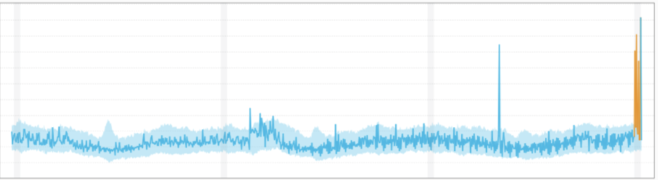
\includegraphics[width=1\textwidth]{images/outlier_type1.png}
\centering
\caption{Globalna anomalija. Preuzeto s  \cite{OutlierAnalysis}}
\label{fig:outlier1}
\end{figure}

\item Kontekstualne anomalije

Kontekstualne ili uvjetne anomalije su opažanja čije se vrijednosti znatno razlikuju od ostalih opažanja koja postoje u istom kontekstu. Takve vrijednosti ne moraju biti izvan globalnih očekivanja, ali odudaraju od konteksta u kojem se nalaze. Također, jedan podatak koji je anomalija u kontekstu jednog skupa podataka ne mora biti anomalija u drugom. Ovakva odstupanja najčešća su u podacima vremenskih serija jer takvi skupovi podataka sadrže zapise ovisne o vremenskom razdoblju. Slika \ref{fig:outlier2} prikazuje primjer takve anomalije.

\begin{figure}[htb]
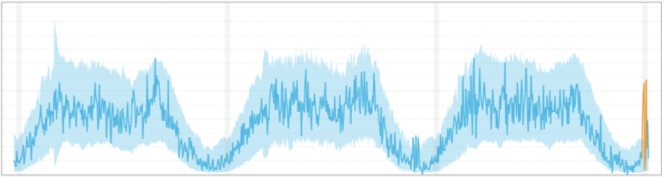
\includegraphics[width=1\textwidth]{images/outlier_type2.png}
\centering
\caption{Kontekstualna anomalija. Preuzeto s  \cite{OutlierAnalysis}}
\label{fig:outlier2}
\end{figure}

\item Kolektivne anomalije

Podskup podataka smatra se kolektivnom anomalijom ako njihove vrijednosti kao grupa značajno odstupanju od cijelog skupa podataka, ali vrijednosti pojedinačnih podataka nisu same po sebi anomalne ni u globalnom ni u kontekstualnom smislu. U podacima vremenskih serija, kolektivne anomalije mogu se manifestirati kao vrhovi i doline koje se javljaju izvan vremenskog okvira kada je takvo ponašanje normalno, kao što se vidi na slici \ref{fig:outlier3}.

\begin{figure}[htb]
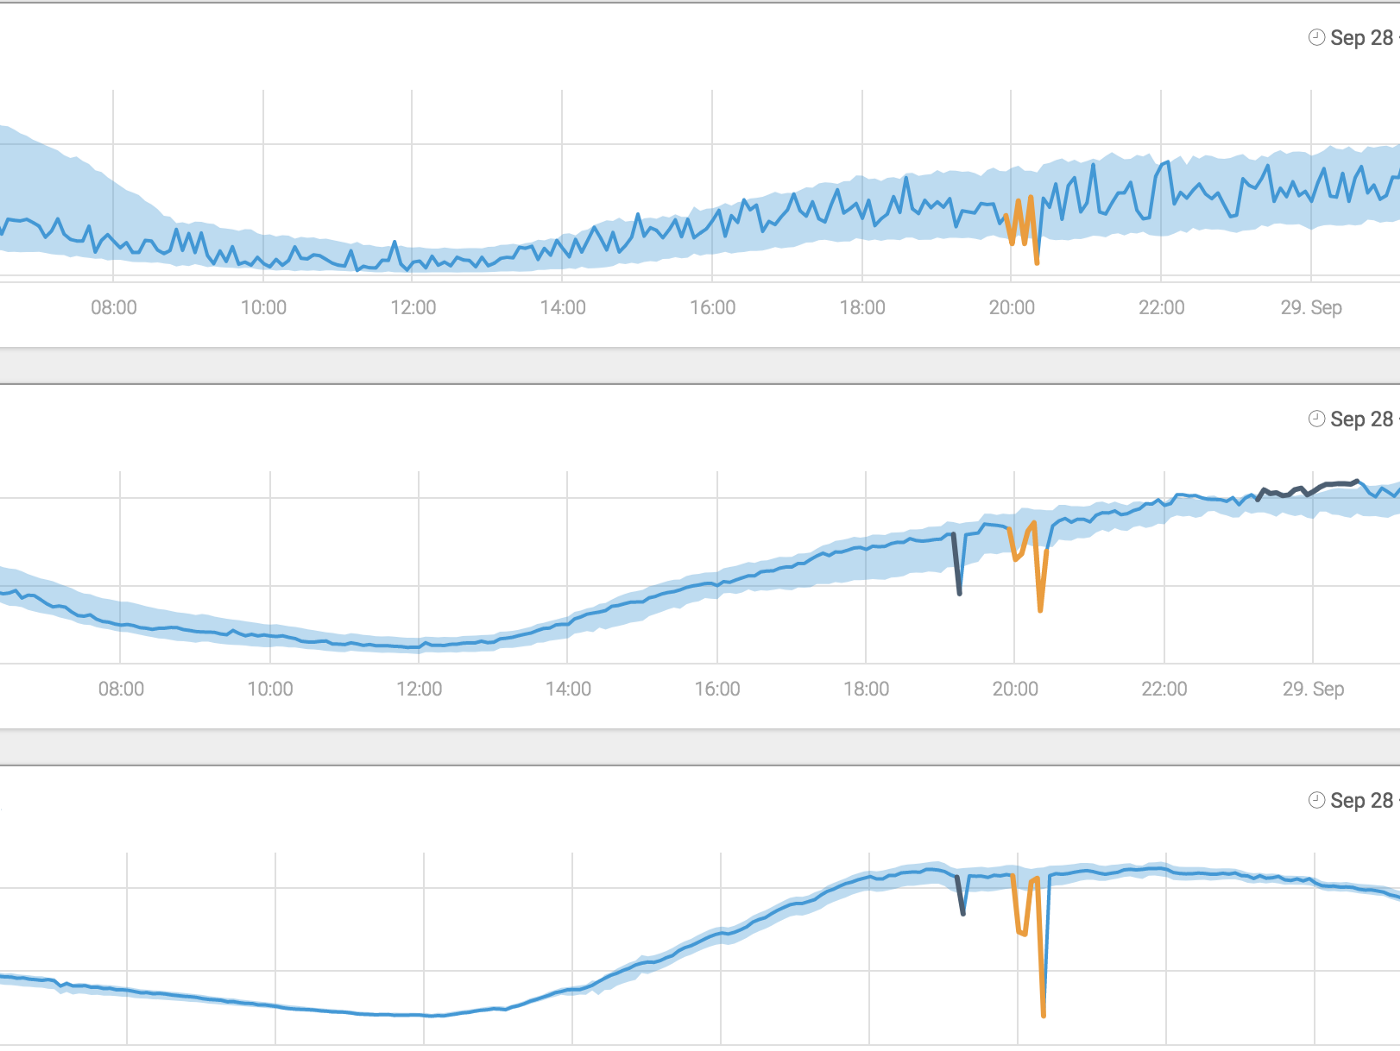
\includegraphics[width=1\textwidth]{images/outlier_type3.png}
\centering
\caption{Kolektivna anomalija. Preuzeto s  \cite{OutlierAnalysis}}
\label{fig:outlier3}
\end{figure}
\end{enumerate}

Ovisno o vrsti anomalije primjenjuju se različite metode i načini detekcije. Ovaj rad fokusira se na globalne anomalije i njihovo pronalaženje.

\section{Problem otkrivanja anomalija}
Otkivanje anomalija svodi se na problem definiranja očekivanog ponašanja podataka ili granica unutar kojih se podaci smatraju normalnima te prepoznavanje točaka koje se ne nalaze unutar njih. Postoji nekoliko faktora koji čine ovaj problem vrlo teškim.

\begin{itemize}
\item Učinkovito modeliranje normalnih vrijednosti i ponašanja može biti vrlo izazovan problem. Često je teško nabrojati sva moguća normalna ponašanja nekog objekta i klasificirati neki podatak kao anomaliju. Također, granica  između normalnih podataka i anomalija može biti vrlo nejasna.
\item Svaki problem zahtjeva specifičan način detekcije anomalija jer su odabir mjere sličnosti i modeliranje odnosa ovisni o svojstvima tog problema. Zbog toga nije moguć razvoj univerzalno primjenjive metode otkivanja anomalija.
\item Prikupljeni podaci često sadrže šum koji može imati vrijednosti koje znatno odstupaju od normalnih ili čak nedostaju. Šum smanjuje kvalitetu podataka i otežava definiranje granica između normalnih podataka i anomalija te se često šum može pogrešno odrediti kao anomalija i obrnuto.
\item Mnogi načini otkrivanja anomalija postaju neučinkoviti u slučaju velike dimenzionalnosti skupa podataka. Podaci su tada rijetki i udaljenosti među podacima su sve veće te se puno točaka može pogrešno klasificirati kao anomalija.
\item U nekim primjenama, korisnik ne želi samo prepoznati anomalije već i razumjeti zašto su ti podaci detektirani kao abnormalni. Zbog toga metoda otkrivanja anomalija mora biti razumljiva, smislena i pružiti opravdanje detekciji.
\end{itemize}

\section{Metode otkrivanja anomalija}
Postoji puno različitih tehnika otkrivanja anomalija i one se mogu podijeliti u četiri glavne kategorije.

\begin{enumerate}
\item Statističke metode

Statistički pristup naziva se još i pristup zasnovan na modelu jer sadrži model koji opisuje obilježja skupa podataka. Model najčešće sadrži distribuciju vjerojatnosti podataka i za svaki podatak računa se vjerojatnost njegova pojavljivanja u tom modelu. Ako je ta vjerojatnost vrlo mala, podatak se proglašava anomalijom.
\item Metode zasnivane na blizini

\begin{enumerate}
\item Metode zasnivane na udaljenosti

Metode zasnivane na udaljenosti pretpostavljaju da je podatak anomalija ako mu se najbliži susjedi nalaze daleko u prostoru značajki odnosno ako blizina njegovih susjeda značajno odstupa od blizine većine drugih objekata njihovim susjedima u istom skupu podataka.
\item Metode zasnivane na gustoći

Metode zasnivane na gustoći koriste broj podataka koji se nalaze unutar definiranog prostora ispitivanog podatka za definiranje lokalne gustoće. Što je lokalna gustoća objekta manja, veća je vjerojatnost da je on anomalija.
\end{enumerate}
\item Metode zasnivane na grupiranju

Metode koje se zasnivaju na grupiranju pretpostavljaju da normalni podaci pripadaju velikim i gustim grupama, dok anomalije pripadaju malim i rijetkim grupama ili ne pripadaju niti jednoj. Razlika između grupiranja i metoda zasnivanih na gustoći je u tome što grupiranje dijeli podatke u grupe dok metode zasnivane na gustoći dijele podatkovni prostor.
\end{enumerate}
U ovom radu za detekciju anomalija koristit će se algoritmi zasnivani na grupiranju. Za usporedbu su izabrani algoritam K-sredina, algoritam DBSCAN i model Gaussove mješavine.


\chapter{Algoritmi grupiranja}
\section{O algoritmima grupiranja}
Grupiranje je podjela skupa podataka u grupe, tako da su podaci u istoj grupi sličniji jedni drugima nego podacima iz ostalih grupa. Cilj jest pronalaženje intrinzičnih grupa u skupu podataka. Algoritmi grupiranja pripadaju u skupinu nenadziranih metoda strojnog učenja jer su ulazni podaci dani bez ciljnih vrijednosti odnosno nisu označeni. 

\subsection{Podjela}
Grupiranje se može podijeliti u dvije kategorije:

\begin{enumerate}
\item Tvrdo grupiranje - podatak ili pripada grupi ili ne pripada
\item Meko grupiranje - podatak pripada svakoj grupi s određenom vjerojatnošću
\end{enumerate}

Osim po tipu grupiranja koje provode, algoritmi grupiranja razlikuju se i po tome kako definiraju pojam grupe i sličnost podataka. Svaki algoritam pretpostavlja specifičan model grupe, a najčešći modeli su:

\begin{enumerate}
\item Modeli povezanosti - na osnovi udaljenosti podataka stvara se hijerarhijsko stablo grupa 
\item Centroidni modeli - podaci se organiziraju u nehijerarhijske grupe ovisno o udaljenosti od centroida te grupe
\item Modeli distribucije - grupe se modeliraju pomoću vjerojatnosti da podaci pripadaju istoj statističkoj distribuciji
\item Modeli gustoće - područja veće gustoće povezuju se u grupe
\end{enumerate}

Ne postoji objektivno najbolji algoritam grupiranja, već odabir algoritma ovisi o problemu koji se rješava. Algoritam se može odabrati na osnovi modela grupe ili eksperimentalno. Također, algoritam dizajniran za jednu vrstu modela grupe općenito neće raditi na skupu podataka koji sadrži drugačiji tip grupa.

U ovom radu uspoređivat će se tri različita modela: algoritam K-sredina kao predstavnik centroidnih modela, DBSCAN algoritam kao model gustoće i model Gaussove mješavine koji pripada modelima distribucije.

\subsection{Vrednovanje}
Rezultati algoritama grupiranja mogu se vrednovati na dva načina. Prvi je vredovanje korištenjem podataka za koje su poznate oznake grupa. Takvo vrednovanje mjeri koliko je dobiveno grupiranje blizu unaprijed određenoj podjeli. Metode vrednovanja tada su često prilagođene varijante metoda koje se koriste za vrednovanje klasifikacije. Neke od tih metrika su:

\begin{enumerate}
\item Matrica zabune (eng. \textit{Confusion Matrix})

Matrica koja opisuje uspješnost modela prikazom broja istinski pozitivnih (eng. \textit{True Positive - TP}), lažno positivnih (eng. \textit{False Positive - FP}), istinski negativnih (eng. \textit{True Negative - TN}) i lažno negativnih (eng.  \textit{False Negative - FP}) primjera.

\item Točnost (eng. \textit{Accuracy})

Točnost je udio točno klasificiranih primjera u skupu svih primjera.
\begin{equation*} \label{eq:accuracy}
Acc = \frac{TP+TN}{TP+TN+FP+FN}
\end{equation*}

\item Preciznost (eng. \textit{Precision})

Preciznost predstavlja udio točno klasificiranih primjera među onima koje je model deklarirao kao pozitivne.
\begin{equation*} \label{eq:precision}
P = \frac{TP}{TP+FP}
\end{equation*}

\item Odziv (eng. \textit{Recall})

Odziv je udio točno klasificiranih primjera u skupu svih stvarno pozitivnih primjera.
\begin{equation*} \label{eq:recall}
R = \frac{TP}{TP+FN}
\end{equation*}

\item F1-mjera (eng. \textit{F1-score})

F1-mjera jest harmonijska sredina preciznosti i odziva i najčešće korištena mjera za usporedbu klasifikatora.
\begin{equation*} \label{eq:f1}
F1 = \frac{2PR}{P+R}
\end{equation*}

\item AUC mjera

ROC krivulja (eng. \textit{Receiver Operating Characteristic curve}) jest graf koji prikazuje odnos stope istiniski pozitivnih primjera (eng. \textit{True Positive Rate - TPR}) odnosno odziva i stope lažno pozitivnih primjera (eng. \textit{False Positive Rate - FPR}), koja se računa kao: 
\begin{math}
\frac{FP}{FP+TN}
\end{math}. Njihov odnos prikazuje se na svim mogućim pragovima klasifikacije. AUC mjera (eng. \textit{Area under the ROC curve}) predstavlja površinu ispod cijele ROC krivulje.

\item Randov indeks

Randov indeks računa u kojoj mjeri dobiveno grupiranje odgovara referentnom grupiranju odnosno točnost na razini parova primjera. Za svaki mogući par iz skupa primjera gleda se jesu li ta dva primjera
završila u istoj grupi ili nisu.
\begin{equation*} \label{eq:rand}
R =  \frac{a+b}{{N \choose 2}}
\end{equation*}
gdje je:
\begin{itemize}
\item \textit{a} - broj jednako označenih parova u istim grupama
\item \textit{b} - broj različito označenih parova u različitim grupama
\end{itemize}

\end{enumerate}

Drugi način vrednovanja algoritama grupiranja jest korištenje metrika koje ne zahtjevaju oznake podataka kako bi izračunale učinkovitost algoritma. Najčešće korištene metrike su:

\begin{enumerate}
\item Koeficijent siluete (eng. \textit{Silhouette Coefficient})

Koeficijent siluete definira se na osnovi udaljenosti unutar grupe i između različitih grupa i računa se kao:
\begin{equation*} \label{eq:silouette}
S = \frac{1}{N}\sum_{i=1}^{N}\frac{b_i-a_i}{max(a_i,b_i)} 
\end{equation*}
gdje je:
\begin{itemize}
\item \textit{a} - srednja udaljenost između uzorka \textit{i} i svih ostalih podataka u toj grupi
\item \textit{b} - srednja udaljenost između uzorka \textit{i} i svih ostalih podataka u drugoj najbližoj grupi
\end{itemize}

Vrijednost koeficijenta siluete nalazi se u skupu \begin{math}[-1,1] \end{math} i što je ona veća, grupe su jasnije odijeljene i grupiranje se smatra točnijim.

\item Dunnov indeks

Dunnov indeks zahtjeva da su udaljenosti primjera unutar grupe male, a udaljenosti između različitih grupa što veće. Računa se kao:
\begin{equation*} \label{eq:silouette}
D = \frac{\min_{1\leq i < j \leq m} \delta(C_i,C_j)}{\max_{1\leq k \leq m} \Delta_k}
\end{equation*}
gdje je:
\begin{itemize}
\item $\delta(C_i,C_j)$ - udaljenost između grupa $C_i$ i $C_j$ (udaljenost između dva najbliža primjera, dva najudaljenija primjera ili prosječna udaljenost)
\item $\Delta_k$ - udaljenost primjera unutar iste grupe (najveća udaljenost između dva primjera, prosječna udaljenost ili udaljenost primjera od centroida grupe)
\end{itemize}

Što je vrijednost Dunnovog indeksa veća, bolje je grupiranje.

\item Davies-Bouldin indeks

Davies-Bouldin indeks računa se kao prosjek sličnosti svake grupe s grupom koja joj je najsličnija: 
\begin{equation*} \label{eq:silouette}
DB = \frac{1}{K}\sum_{i = 1}^{K} \max_{j\neq i} \frac{\Delta_i + \Delta_j}{\delta(C_i,C_j)}
\end{equation*}

Razlikuje se od ostalih metrika jer manja vrijednost ovog indeksa označava bolje grupiranje.

\item DBCV (eng. \textit{Density-Based Clustering Validation})

Metrika DBCV računa gustoću unutar grupe i gustoću između grupa. Visoka gustoća unutar grupe, a niska gustoća između njih ukazuje na dobro grupiranje.

\end{enumerate}

Za vrednovanje algoritama u ovom radu koristit će se sve navedene metode osim točnosti, Dunnovog indeksa i metode DBCV. Točnost je nepouzdana u slučaju neuravnoteženih razreda kao što je to slučaj u detekciji anomalija, a Dunnov indeks i DBCV su metode bez svojstva razmjernog rasta, čije računanje postaje računski vrlo zahtjevno već za nekoliko tisuća primjera.

\section{Algoritam K-sredina}
Algoritam K-sredina (eng. \textit{K-Means}) najpoznatiji je algoritam grupiranja koji se zasniva na centroidnom modelu. U ovom algoritmu, svaka grupa ima centroid koji se računa kao srednja vrijednost članova grupe i predstavlja tu grupu. Primjeri se iz neoznačenog skupa podataka grupiraju u $K$ grupa na način da svaki podatak pripada onoj grupi čijem je centroidu najbliži. 

Algoritam očekuje broj grupa $K$ kao hiperparameter i njegova se vrijednost može odrediti na više načina, a najpoznatiji su:
\begin{itemize}
\item Metoda lakta (eng. \textit{Elbow method})

U metodi lakta grafički se prikazuje ovisnost funkcije gubitka o broju grupa $K$. S porastom broja grupa vrijednost funckije će se smanjivati te je cilj pronaći ``lakat'' funkcije, odnosno broj grupa nakon kojeg se vrijednosti funkcija počinju smanjivati vrlo sporo.

\item Analiza siluete (eng. \textit{Silhouette analysis})

Ova je metoda grafička metoda koja se zasniva na ranije objašnjenom koeficijentu siluete. Njegova vrijednost prikaže se za svaki primjer iz skupa podataka ovisno o grupi u koju je primjer raspoređen te se izabere onaj broj grupa za koji svi primjeri imaju približno jednak koeficijent siluete.

\end{itemize}

Osim odabira broja grupa, potrebno je definirati i način odabira početnih centroida. Neki od mogućih prisupa su:
\begin{itemize}
\item Nasumičan odabir $K$ primjera.
\item Nasumična dodjela grupe svakom primjeru i izračun centroida na osnovi primjera u grupi.
\item Izračun srednje vrijednosti sviju primjera i dodavanje $K$ slučajnih vektora toj vrijednosti.
\item Nasumičan odabir prvog centroida, nakon čega se svaki sljedeći bira na način da bude što dalje od postojećih. Verzija algoritma koja ostvaruje ovakav pristup zove se \textit{K-sredine++}.

\end{itemize}

Postupak grupiranja algoritma K-sredina je iterativan. Nakon inicijalizacije početnih centroida, svi se primjeri stavljaju u onu grupu čiji im je centroid najbliži. U sljedećem se koraku, na osnovi razvrstanih primjera, ponovno računaju novi centroidi za svaku grupu. Dalje se ponavljaju ova dva koraka sve do konvergencije odnosno do trenutka kad više nema promjene u podjeli primjera grupama i u vrijednostima centroida. Ovaj postupak prikazan je pseudokodom \ref{alg:kmeans} i na slici \ref{fig:kmeans}.

 \begin{lstlisting}[caption = Pseudokod algoritma K-sredina, label = {alg:kmeans}, escapeinside={*}{+}]
 definiraj broj grupa *$K$+
 inicijaliziraj centroide *$\mu_k$+, *$k = 1, ..., K$+
 ponavljaj
 	za svaki *$x_i \in D$+
 		pronađi najbliži centroid
 		dodjeli *$x_i$+ toj grupi
	za svaki *$\mu_k$+, *$k = 1, ..., K$+
		ažuriraj vrijednost centroida
 dok svi *$\mu_k$+ ne konvergiraju
\end{lstlisting}

\begin{figure}
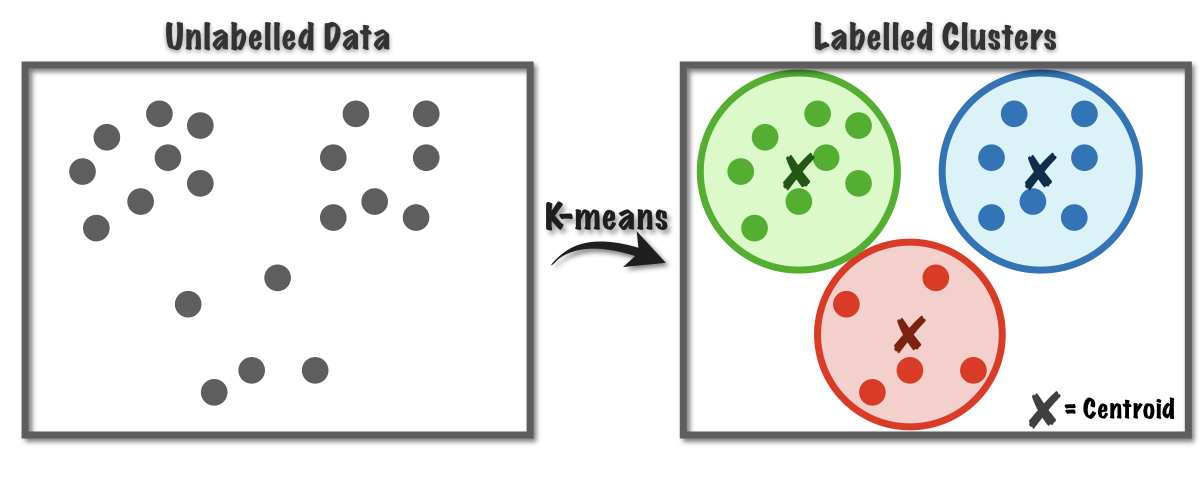
\includegraphics[width=0.9\textwidth]{images/kmeans.png}
\centering
\caption{Primjer izvođenja algoritma K-sredina uz $K = 3$. Preuzeto s  \cite{kMeansUsingPython}}
\label{fig:kmeans}
\end{figure}

Bitna karakteristika algoritma K-sredina je da pripada algoritmima tvrdog grupiranja, što znači da će svaku točku dodijeliti jednoj i točno jednoj grupi. Algoritam se dobro nosi s velikim skupovima podataka jer ima linearnu vremensku složenosti $O(nkdi)$, gdje je:
\begin{itemize}
\item n - veličina skupa podataka
\item k - broj grupa
\item d - dimenzionalnost podataka
\item i - broj iteracija algoritma
\end{itemize}

Međutim, algoritam K-sredina uvijek traži grupe sfernog oblika te ne može prepoznati nekonveksne grupe. Također, jako je osjetljiv na prisutnost anomalija i šuma u podacima.

\section{DBSCAN algoritam}
DBSCAN algoritam (eng. \textit{Density-based spatial clustering of applications with noise}) priprada u skupinu algoritama grupiranja zasnivanih na gustoći. On grupira zajedno točke koje su blizu jedna drugoj odnosno točke s mnogo susjednih točaka. Primjere koji nisu svrstani niti u jednu grupu i nalaze se u područjima niske gustoće algoritam označava kao anomalije. Kao i algoritam K-sredina, i DBSCAN je algoritam tvrdog grupiranja.

Glavna ideja algoritma DBSCAN jest da grupa mora sadržavati određeni minimalni broj točaka unutar definiranog polumjera. Zato algoritam zahtjeva dva parametra: 
\begin{enumerate}
\item \textit{minPts} 

Parametar \textit{minPts} predstavlja najmanji broj točaka u grupi da bi se ona smatrala gusto popunjenom. Za njegovu procjenu može se primjeniti generalno pravilo $minPts \geq D + 1$, gdje je $D$ broj dimenzija skupa podataka. Također, što je veći skup podataka potrebno je odabrati veći \textit{minPts} i tada se može koristiti pravilo $minPts = 2*D$. Veće vrijednosti obično daju bolje rezultate kada je u podacima prisutan šum.
\item $\epsilon$

Parametar $\epsilon$ jest polumjer unutar kojeg se traže susjedne točke. Pri odabiru vrijednosti $\epsilon$ nema generalnog pravila. Vrijednost ne smije biti ni prevelika niti premala i mora biti sukladna udaljenostima među podacima. 
\end{enumerate}

DBCAN algoritam pridjeljuje svakoj točki jednu od tri moguće oznake:
\begin{enumerate}
\item Središnja točka (eng. \textit{Core point}) - točka oko koje se nalazi minimalno \textit{minPts} drugih točaka unutar udaljenosti $\epsilon$
\item Granična točka (eng. \textit{Border point}) - točka koja ima barem jednu središnju točku na udaljenosti manjoj od $\epsilon$, ali nalazi se na rubu grupe i broj točaka oko nje manji je od \textit{minPts} 
\item Točka šuma (eng. \textit{Noise point}) - točka koja nije niti središnja niti granična točka; točka od koje DBSCAN nije znao formirati grupu te je proglašava anomalijom
\end{enumerate}

Na slici \ref{fig:dbscan-points} prikazane su grafički različite vrste točaka.

\begin{figure}[htb]
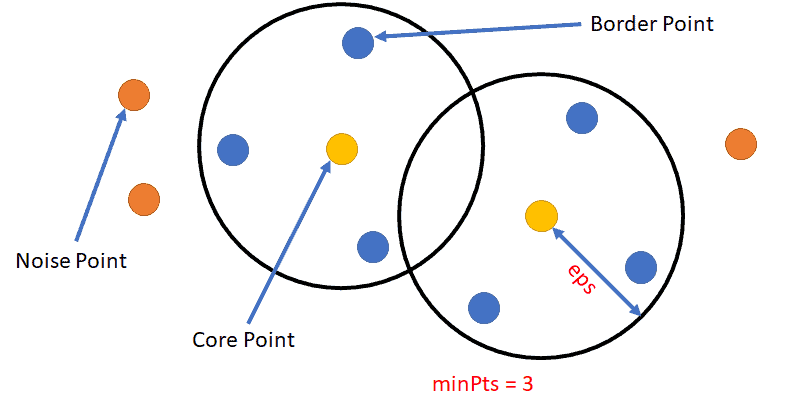
\includegraphics[width=0.8\textwidth]{images/dbscan-points.png}
\centering
\caption{Primjer središnje točke, granične točke i točke šuma uz $minPts$ = 3. Preuzeto s  \cite{DBSCANClustering}}
\label{fig:dbscan-points}
\end{figure}

Središnja točka $p$ formira grupu zajedno sa svim središnjim i graničnim točkama koje su iz nje dohvatljive. Točka $q$ može biti:
\begin{itemize}
\item Izravno dohvatljiva - ako se nalazi unutar udaljenosti $\epsilon$ od točke $p$
\item Dohvatljiva - ako postoji put $p_1, ..., p_n$, pri čemu je $p_1 = p$ i $p_n = q$ i svaka točka $p_{i+1}$ izravno je dohvatljiva iz točke $p_i$
\end{itemize}

Dohvatljivost nije simetrična relacija, već samo središnje točke mogu dohvatiti granične. Zbog toga je uveden pojam povezanosti, kojim se formalno definira opseg grupe. Dvije točke $p$ i $q$ povezane su ako postoji točka $o$ takva da su i $p$ i $q$ dohvatljive iz $o$. Ova relacija je simetrična i grupa tada ispunjava sljedeća svojstva:
\begin{itemize}
\item Sve točke unutar grupe međusobno su povezane.
\item Ako je točka dohvatljiva iz bilo koje točke koja pripada grupe, tada ona također pripada grupi.
\end{itemize}

Svojstva izravne dohvatljivosti, dohvatljivosti i povezanosti prikazana su grafički na slici \ref{fig:dbscan-dohvatljivost}.

\begin{figure}[htp]
\begin{subfigure}{.3\textwidth}
\centering
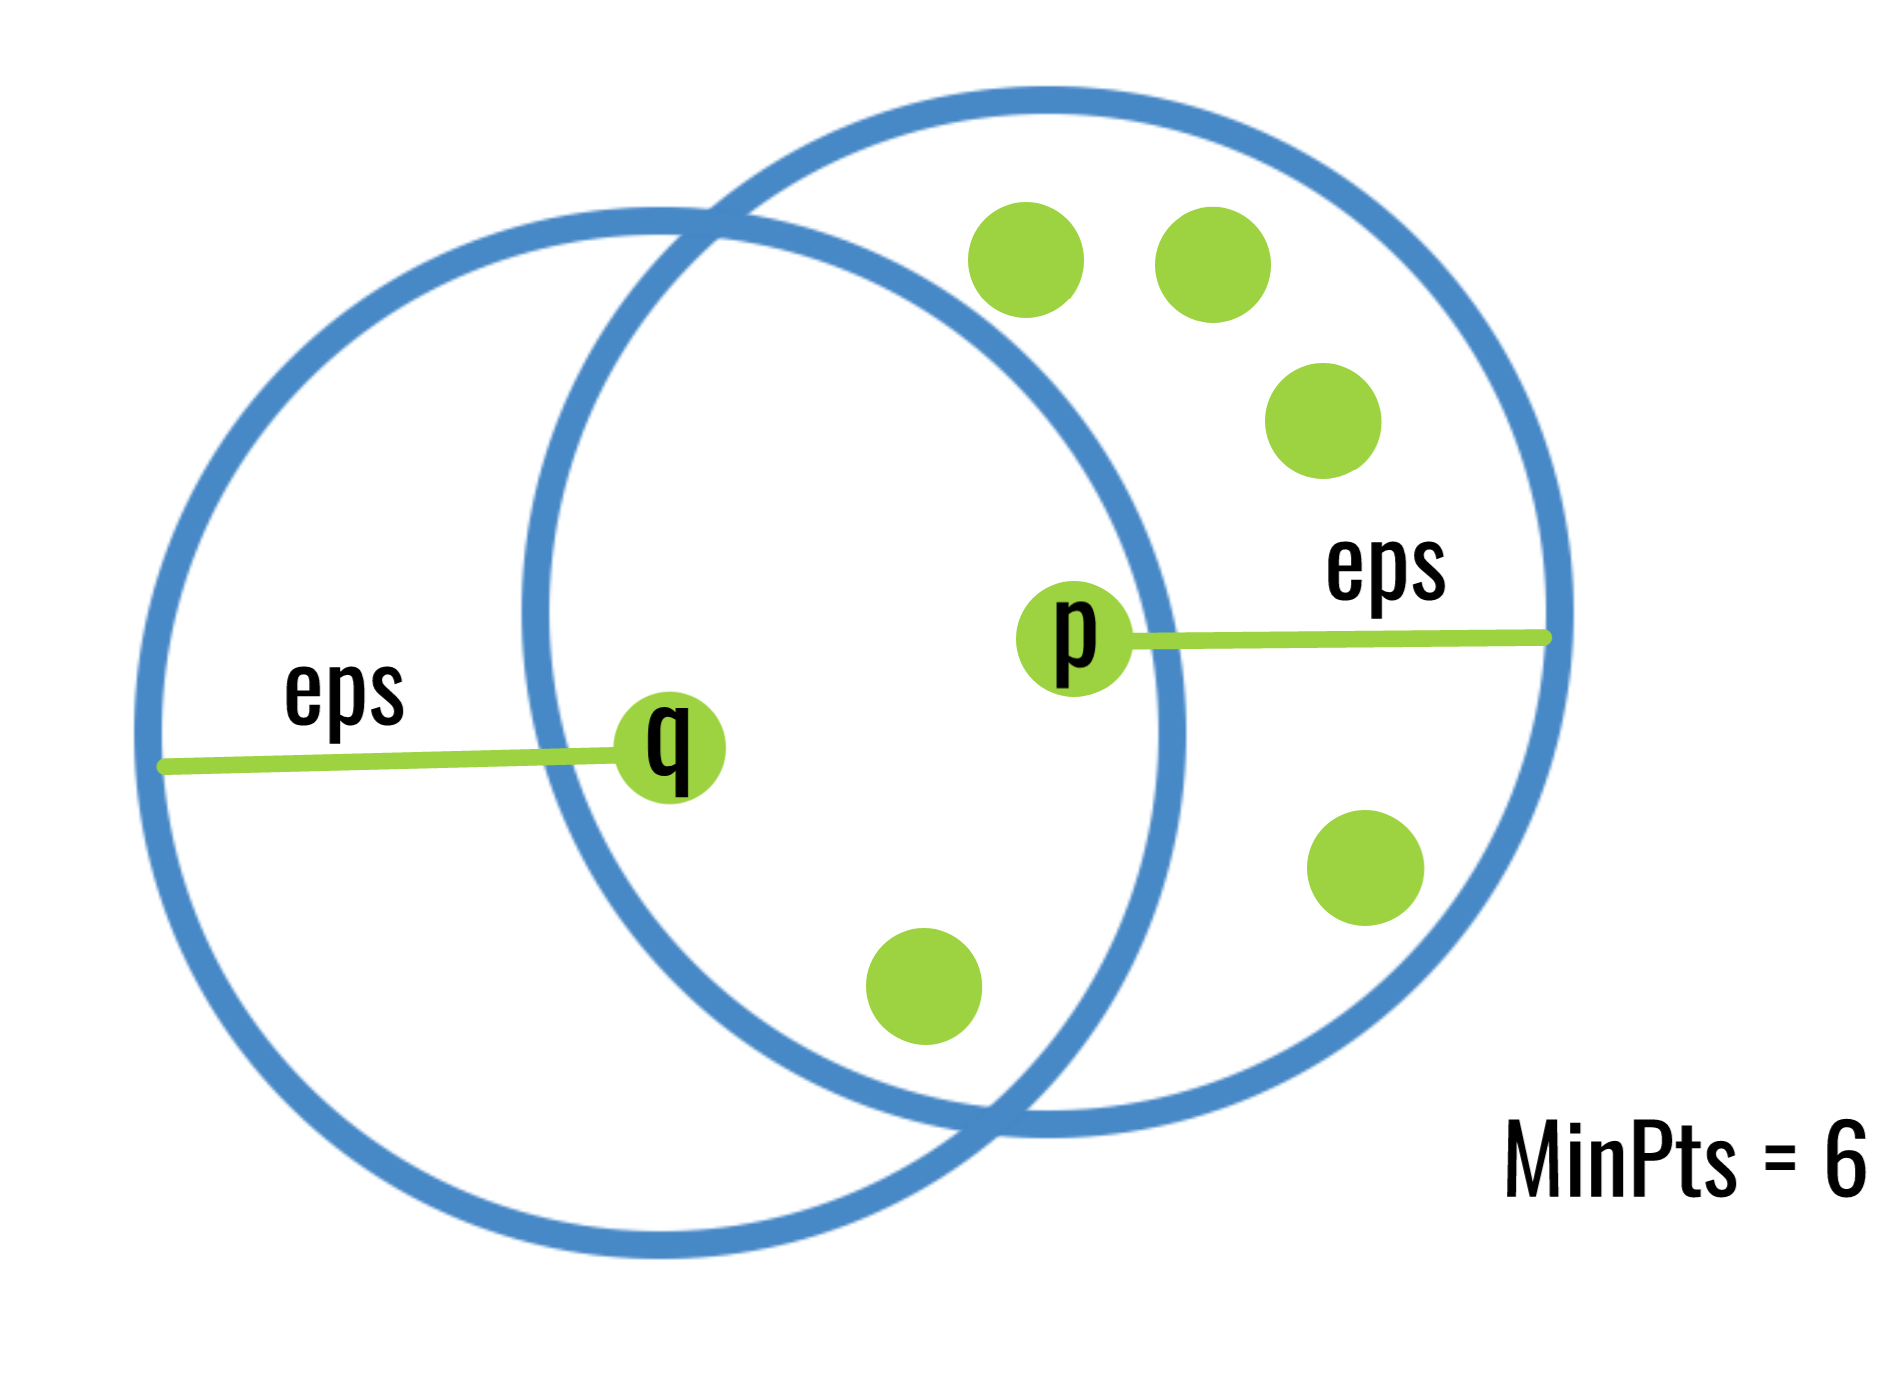
\includegraphics[width=1\textwidth]{images/dbscan1.png}
\caption{Točka $q$ je izravno dohvatljiva iz točke $p$}
\end{subfigure}
\begin{subfigure}{.3\textwidth}
\centering
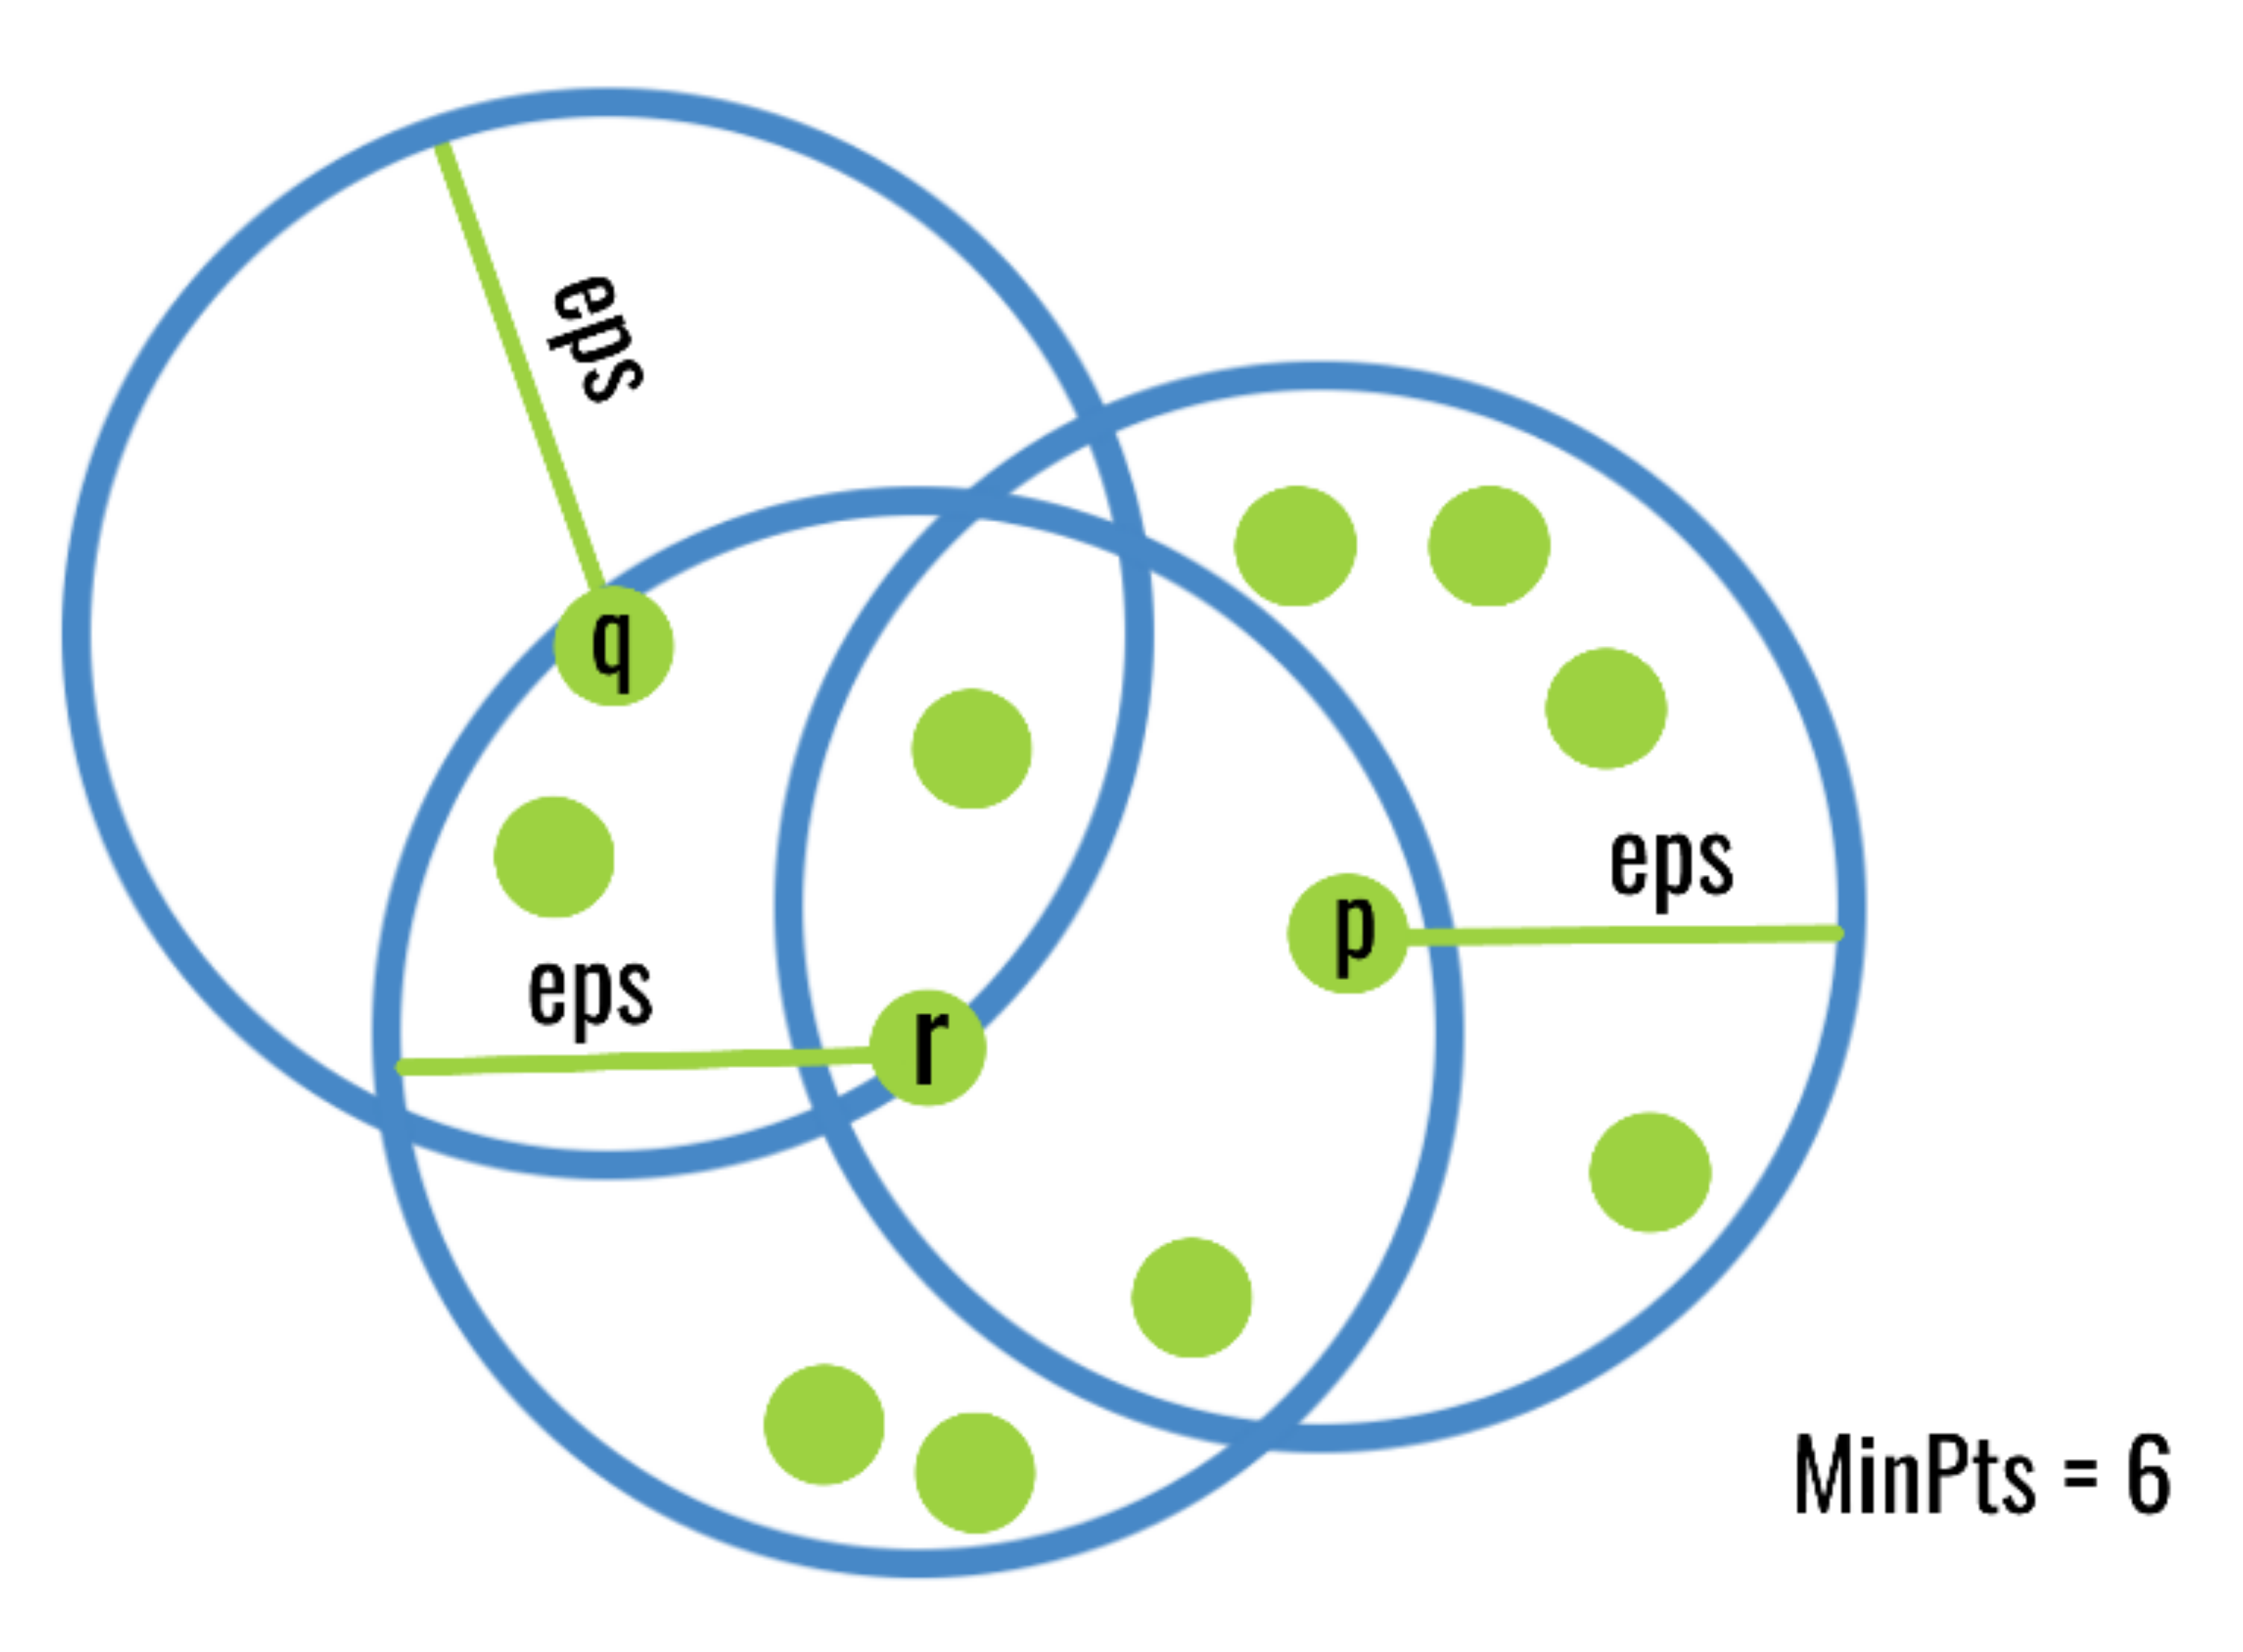
\includegraphics[width=1\textwidth]{images/dbscan2.png}
\caption{Točka $q$ je dohvatljiva iz točke $p$ preko točke $r$}
\end{subfigure}
\begin{subfigure}{.3\textwidth}
\centering
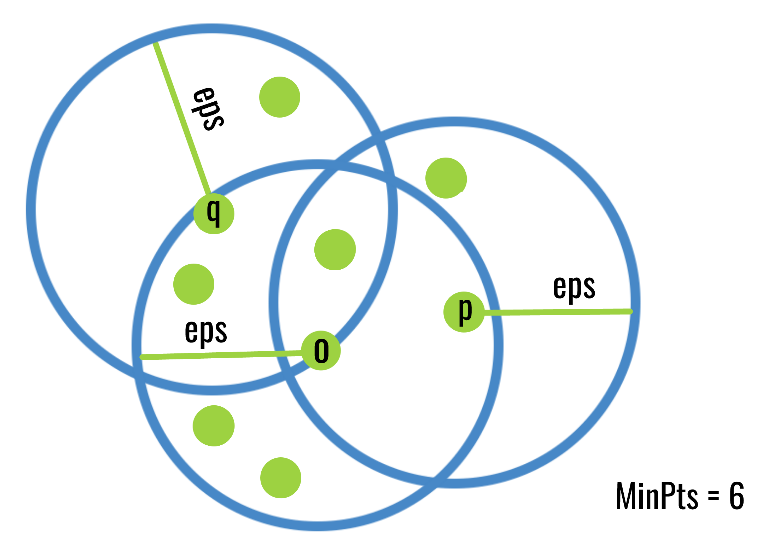
\includegraphics[width=1\textwidth]{images/dbscan3.png}
\caption{Točka $p$ i točka $q$ su povezane preko točke $o$}
\end{subfigure}
\caption{Prikaz izravne dohvatljivosti, dohvatljivosti i povezanosti na primjeru gdje je $minPts = 6$. Slike su preuzete s \cite{DBSCANReachability}}
\label{fig:dbscan-dohvatljivost}
\end{figure}

Na početku algoritma odabire se nasumična točka od koje se formira grupa ako ona ispunjava navedeni kriterij. Grupe se zatim rekurzivno proširuju obilaženjem ostalih članova grupe. Kad se grupa više ne može proširiti, odabire se nasumično nova točka iz skupa podataka i algoritam se ponavlja dok sve točke nisu obiđene. Pseudokod \ref{alg:dbscan} prikazuje pseudokod algoritma DBSCAN.

\begin{lstlisting}[caption = Pseudokod algoritma DBSCAN, label = {alg:dbscan}, escapeinside={*}{-}]
 definiraj minimalan broj članova grupe *$minPts$- i udaljenost *$\epsilon$-
 inicijaliziraj početni broj grupa: *$C = 0$-
 za svaku točku *$p \in D$-
 	ako je točka *$p$- već označena
       		nastavi
    	pronađi skup točaka *$S$- izravno dohvatljivih iz *$p$-
    	ako je *$|S| < minPts$- onda 
 		označi *$p$- kao točku šuma
 	   	nastavi
 	*$C = C + 1$-
 	dodaj *$p$- u grupu *$C$-
	za svaku točku *$q \in S$-
	  	ako točka *$q$- već pripada grupi
	  		nastavi
	      	dodaj *$q$- u grupu *$C$-
	      	pronađi skup točaka *$N$- izravno dohvatljivih iz *$q$-
	      	ako je *$|N| \geq minPts$- onda 
	         	dodaj točke iz *$N$- u skup *$S$-

\end{lstlisting}

Ako je skup podataka spremljen tako da se upiti o susjedstvu mogu izvoditi u logaritamskom vremenu, složenost DBSCAN algoritma je $O(n log n)$, gdje je $n$ broj podataka. Ako nema strukture indeksiranja, složenost raste na $O(n^2)$.

Prednosti algoritma DBSCAN su što ne zahtjeva definiranje broja grupa unaprijed, može pronaći grupe proizvoljnog oblika i otporan je na prisutnost šuma i anomalija. Nedostatak mu je što ne može dobro grupirati skup podataka u kojem je prisutna velika razlika u gustoći među grupama jer se tada ne može odabrati kombinacija parametara \textit{minPts} i $\epsilon$ koja bi bila prikladna za sve grupe. 

\section{Model Gaussove mješavine}

Gaussova je mješavina model distribucije koji pretpostavlja da su sve točke iz skupa podataka stvorene iz mješavine konačnog broja Gaussovih distribucija s nepoznatim parametrima. Model zatim grupira podatke na način da svaka grupa sadrži podatke iz jedne distribucije.

Gaussova distribucija još se naziva normalnom distribuciju i ima karakterističan zvonolik oblik. Funkcija gustoće vjerojatnosti Gaussove distribucije u jednoj dimenziji glasi:
\begin{equation} \label{eq:gauss1}
\mathcal{N}(x;\mu,\sigma) = \frac{1}{{\sigma \sqrt {2\pi } }}e^{\frac{-(x - \mu)^2 }{2\sigma ^2 }}
\end{equation}

pri čemu je:
\begin{itemize}
\item $\mu$ - srednja vrijednost skupa podataka; određuje ``visinu'' krivulju
\item $\sigma$ - standardna devijacija podataka; odeđuje ``širinu'' krivulje
\end{itemize}

Funkcija gustoće vjerojatnosti daje vjerojatnost dobivanja podatka $x$ u slučaju kada imamo normalnu distribuciju s parametrima $\mu$ i $\sigma$. Slika \ref{fig:gauss1} prikazuje funkciju gustoće za različite vrijednosti parametara $\mu$ i $\sigma$.

\begin{figure}[htb]
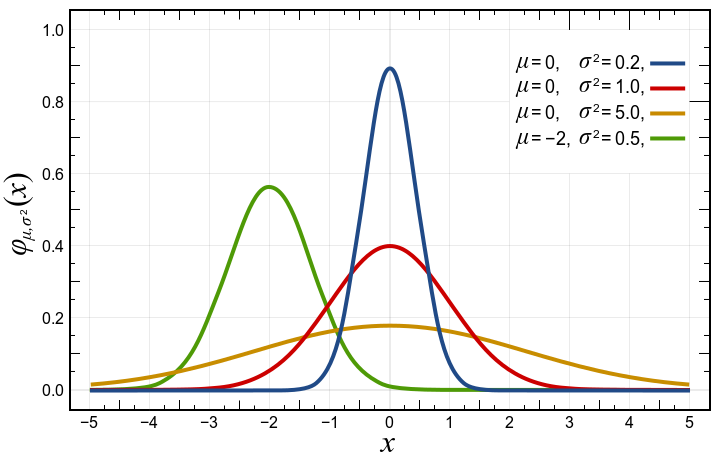
\includegraphics[width=0.8\textwidth]{images/gauss1.png}
\centering
\caption{Funkcija gustoće vjerojatnosti Gaussove distrubucije za različite vrijednosti parametara $\mu$ i $\sigma$. Preuzeto s  \cite{normalDistWiki}}
\label{fig:gauss1}
\end{figure}

U slučaju više dimenzionalnog skupa podataka, formula multivarijatne (višedimenzijske) Gaussove razdiobe glasi:

\begin{equation}
\mathcal{N}(X;\mu,\Sigma)  =\frac{1}{\sqrt{(2\pi)^{k}|\Sigma|}}e^{-\frac{1}{2}(X-\mu)^T\Sigma^{-1}(X-\mu)}
\end{equation}

U tom je slučaju $k$ broj dimenzija skupa podatka, $\mu$ $k$-dimenzionalni vektor srednjih vrijednosti, a $\Sigma$ kovarijacijska matrica veličine $k \times k$. Kovarijacijska matrica prikazuje, osim varijance svake dimenzije podatka, i odnos između različitih dimenzija.

Gaussova je mješavina funkcija koja se sastoji od onoliko Gaussovih funkcija koliko ima grupa u skupu podataka. Broj grupa $K$ jest hiperparametar algoritma. Svaka Gaussova funkcija u mješavini ima sljedeće parametare:

\begin{itemize}
\item Srednju vrijednost $\mu$ koja definira središte.
\item Kovarijancu $\Sigma$  koja odeđuje ``širinu'' funckije.
\item Vjerojatnost miješanja $\pi$ koja definira vjerojatnosti pripadnosti primjera toj distribuciji.
\end{itemize}

Slika \ref{fig:gauss-mixture} prikazuje kako model Gaussove mješavine grupira podatke u slučaju kada imamo tri grupe.

\begin{figure}[htb]
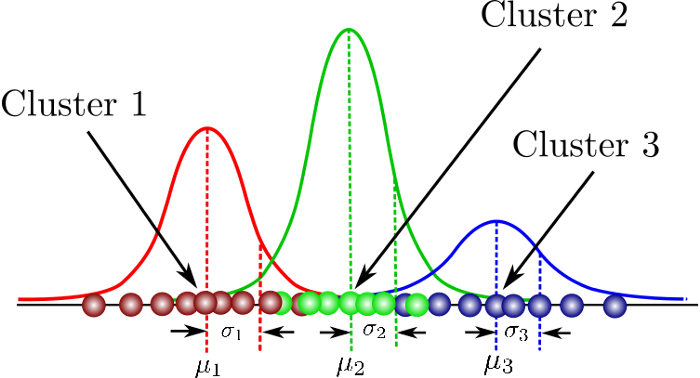
\includegraphics[width=0.8\textwidth]{images/gauss_mixture.png}
\centering
\caption{Primjer Gaussove mješavine za $K = 3$. Preuzeto s  \cite{GaussianMixtureExplained}}
\label{fig:gauss-mixture}
\end{figure}

Model Gaussove mješavine radi na načelu generativnog modeliranja i pretpostavlja se da se ulazni podaci ravnaju po Gaussovoj distribuciji. Iako to nije uvijek slučaj, centralni granični teorem iz statistike kaže da ako se prikuplja sve više i više uzoraka iz skupa podataka, oni imaju tendenciju nalikovati Gaussovoj funkciji, čak i kad izvorna distribucija skupa podataka nije Gaussova.

Cilj ovog modela jest pronaći parametre Gaussove funkcije koji maksimiziraju vjerojatnost dobivanja tih podataka. Svaku točku promatra se kao mješavinu više različitih Gaussovih funkcija te ona ima vjerojatnost:

\begin{equation}\label{eq:prob}
p(x_i) = \sum_{k=1}^{K}\pi_k \mathcal{N}(x_i;\mu_k,\Sigma_k)
\end{equation}
\begin{equation}\label{eq:mixture_prob}
\sum_{k=1}^{K}\pi_k  = 1
\end{equation}

Jednadžba \ref{eq:prob} govori da je određena točka $x$ linearna kombinacija $K$ Gaussovih funkcija. $p(x_i)$ još se naziva i izglednost primjera $x_i$ (eng. \textit{likelihood}). Varijabla $\pi$ predstavlja vjerojatnost miješanja te Gaussove funkcije odnosno njenu jačinu. Ograničenje na vjerojatnosti miješanja jest da njihova suma mora biti 1, kao što se vidi u jednadžbi \ref{eq:mixture_prob}. Cilj algoritma jest maksimizirati logaritamsku izglednost svih podataka u skupu veličine $N$ koja glasi:
\begin{equation}\label{eg:likelihood}
\ln p(X; \mu, \sigma, \pi) = \sum_{i=1}^{N} p(x_i)
 \end{equation}

Potrebno je za svaku Gaussovu funkciju odrediti vrijednosti vjerojatnosti miješanja $\pi_k$, srednje vrijednosti $\mu_k$ i kovarijance $\Sigma_k$, takve da maksimiziraju izraz \ref{eg:likelihood}. Vrijednosti ovih parametara dobiju se primjenom algoritma Očekivanje-Maksimizacija (eng. \textit{Expectation-Maximization Algorithm - EM}). Taj algoritam ima dva koraka:
\begin{enumerate}
\item Očekivanje

U prvoj iteraciji algoritma inicijaliziraju se vrijednosti parametara slučajnim odabirom ili pomoću rezultata grupiranja nekog drugog algoritma. Zatim se u ovom koraku računa vjerojatnost da je svaki podatak stvoren svakom od $K$ Gaussovih funkcija. Vjerojatnost da je primjer $x_i$ stvoren pomoću Gaussove funkcije $j$ računa se kao:
\begin{equation}\label{eq:expectation}
W_{ij} = \frac{\pi_j \mathcal{N}(x_i;\mu_j,\Sigma_j)}{\sum_{k=1}^{K} \pi_k \mathcal{N}(x_i;\mu_k,\Sigma_k)}
\end{equation}

Dijeljenje s $p(x_i)$ provodi se radi normalizacije odnosno kako bi suma svih vjerojatnosti bila 1. U algoritmu K-sredina ovaj korak algoritma odgovara podjeli primjera u grupe.
\item Maksimizacija

Korak maksimizacije ažurira vrijednosti vjerojatnosti miješanja, srednje vrijednosti i kovarijance na sljedeći način:
\begin{equation}\label{eq:max}
\pi_j = \frac{1}{N}\sum_{i=1}^{N} W_{ij}
\end{equation}
\begin{equation}\label{eq:max}
\mu_j = \frac{\sum_{i=1}^{N} W_{ij}x_i}{\sum_{i=1}^{N} W_{ij}}
\end{equation}
\begin{equation}\label{eq:max}
\Sigma_j = \frac{\sum_{i=1}^{N} W_{ij}(x_i-\mu_j)(x_i-\mu_j)^T}{\sum_{i=1}^{N} W_{ij}}
\end{equation}

Vjerojatnost $\pi_j$ računa se kao vjerojatnost da je svaka točka stvorena Gaussovom funkcijom $j$ podijeljeno s ukupnim brojem točaka. Parametri $\mu_j$ i $\Sigma_j$ računaju se kao srednja vrijednost i kovarijacija svih točaka koje su pomnožene s vjerojatnošću $W_{ij}$. Ovaj korak analogan je pomicanju centroida grupa u algoritmu K-sredina.

\end{enumerate}

Ova dva koraka ponavljaju se do konvergencije logaritmske izglednosti podataka, a pseudokod je dan kao pseudokod \ref{alg:gauss}. 

\begin{lstlisting}[caption = Pseudokod modela Gaussove mješavine, label = {alg:gauss}, escapeinside={*}{-}]
 definiraj broj grupa *$K$-
 inicijaliziraj parametre *$\pi$-, *$\mu$- i *$\Sigma$-
 ponavljaj
    za svaku točku *$x_i \in N$-
       za svaku distribuciju *$k \in K$-
	   izračunaj vjerojatnost *$W_{ik}$- da je *$x_i$- nastao iz *$k$-
    za svaku distribuciju *$k \in K$-
       ažuriraj vjerojatnost miješanja *$\pi_{k}$-
       ažuriraj srednju vrijednost *$\mu_{k}$-
       ažuriraj kovarijancu *$\Sigma_{k}$-
dok *$\ln p(X; \mu, \sigma, \pi)$- ne konvergira 

\end{lstlisting}

Model Gaussove mješavine model je mekog grupiranja i svakoj točki dodijeljuje vektor vjerojatnosti pripadanja svakoj grupi. Iako sporije konvergira od algoritma K-sredina, za razliku od njega može se koristiti i na malim skupovima podataka te kada grupe nisu jasno razdvojene. Također, može pronaći grupe različitih oblika i otporan je na prisutnost anomalija ili loše definiranih podataka.

\chapter{Korišteni skupovi podataka}
\section{Otkrivanje prijevare s kreditnim karticama}
Važno je da banke mogu prepoznati neobične transakcije kreditnim karticama kako bi se otkrila prijevara i spasili novci korisnika. Prvi skup podataka koristi se za otkrivanje prijevara kreditnim karicama (eng. \textit{Credit Card Fraud Detection}) i preuzet je s \cite{pang2021deep}. Sadrži transakcije koje su europski vlasnici kartica izvršili kreditnim karticama u rujnu 2013. godine u 2 dana. Skup podataka izrazito je neuravnotežen te prijevare čine samo 0,172\% svih transakcija.

Skup podataka sadrži numeričke značajke koje su rezultat analize glavnih komponenata (eng. \textit{Principal component analysis}). Zbog povjerljivosti nisu dostupni originalni podaci i imena značajki već samo rezultat PCA transformacije. Dobivene glavne komponente su značajke V1, V2, ..., V28. Značajke koje nisu transformirane i koje su zadržale svoje vrijednosti i ime su značajke \textit{Vrijeme} i \textit{Iznos}. Značajka \textit{Vrijeme} sadrži sekunde koje su protekle između svake transakcije i prve transakcije u skupu podataka, a značajka \textit{Iznos} je iznos transakcije. Na kraju, značajka \textit{Klasa} je varijabla oznake koja poprima vrijednost 1 u slučaju prijevare, a 0 inače.

Skup podataka koji se koristi već je obrađen, maknuta je značajka \textit{Vrijeme} jer ne pomaže u problemu detekcije prijevara i provedena je normalizacija podataka.

\section{Detekcija upada u mrežu}
Skup podataka \textit{KDD Cup 1999} umjetno je stvoren skup koji se može koristiti za detekciju mrežnog upada ili napada. Taj skup podataka korišten je za Treće međunarodno natjecanje u otkrivanju znanja i alatima za rudarenje podataka. Zadatak natjecanja bio je izgraditi prediktivni model koji će detektirati upade u mrežu i razlikovati ih od normalnih veza. Svaka veza je slijed TCP paketa koji počinje i završava u nekom definiranom vremenu, u kojem se podaci šalju od izvorne IP adrese na ciljnu IP adresu prema nekom definiranom protokolu.

Ovaj skup podataka sadrži standardni skup podataka za provjeru modela i preuzet je s  \cite{pang2021deep}. Nastao je tako što je \textit{Lincoln Labs} postavio okolinu za prikupljanje neobrađenih TCP podataka za lokalnu mrežu (LAN) tokom devet tjedana simulirajući tipični LAN američkih zračnih snaga. Upravljali su LAN-om kao da se radi o pravoj okolini zračnih snaga uz dodatak višestrukih napada. Prikupljeno je oko 7 milijuna zapisa veza, pri čemu svaka veza ima 41 značajku i označena je kao normalna veza ili kao napad, s točno specificiranom vrstom napada. U skupu za treniranje korišteno je ukupno 24 različita tipa napada.

Za potrebe ovog rada korištena su dva podskupa skupa podataka \textit{KDD Cup 1999}: \textit{U2R} i \textit{Probe}.

Napad \textit{U2R} (eng. \textit{User to Root}) jest napad u kojem napadač na početku pristupa normalnom korisničkom računu, a kasnije dobiva pristup korijenskom korisniku (eng. \textit{root}) iskorištavanjem ranjivosti sustava ili greške korisnika. \textit{Probe} napad skenira mrežu sa svrhom praćenja mreže ili prikupljanje podataka o mreži i mrežnoj aktivnosti.

Novi skupovi podataka izvedeni su iz skupa podataka \textit{KDD Cup 1999} koristeći \textit{U2R} ili \textit{Probe} napad kao anomaliju naspram normalnih veza. Ti skupovi su znatno manji i broj značajki smanjen je na 6 osnovnih: 
\begin{enumerate}
\item Vrsta transportnog protokola
\item Vrsta aplikacijskog protokola
\item Zastavica odnosno status povezivanja
\item Prijava uspješna
\item Prijava ostvarena kao domaćin
\item Prijava ostvarena kao gost
\end{enumerate}

Prve tri značajke su kategoričkog tipa, a druga tri tipa boolean (točno/netočno).

\section{Detekcija raka}
Jedna od važnih primjena otkrivanja anomalija jest u medicini gdje one mogu signalizirati pojavu bolesti. Detekcija anomalija korisiti se za analizu medicinskih slika kako bi se otkrile abnormalne stanice ili tumori. Primjer toga jest predikcija je li tumor dojke dobroćudan ili zloćudan i za tu svrhu korišten je skup podataka preuzet s \cite{Dua:2019}.

Svaki primjer skupa podataka ima 32 značajke, među kojima su i značajke \textit{Identifikacijski broj} i \textit{Dijagnoza}, koja klasificira tumor kao dobroćudni ili zloćudni. Preostale značajke su zračunate iz digitalizirane slike aspiracijske biopsije finom iglom (FNA) tkiva dojke i opisuju karakteristike staničnih jezgri prisutnih na slici. Za svaku jezgru izračunato je deset vrijednosti kao što su radijus, tekstura, područje i glatkoća. Značajke su zatim dobivene iz tih podataka kao srednja vrijednost, standardna pogreška i najgora (odnosno najveća) vrijednost mjerenja. 

Pregled svih korištenih skupova podataka dan u tablici \ref{tab:datasets}.

\begin{table}[h!]
  \begin{center}
    \caption{Podaci o korištenim skupovima podataka.}
    \label{tab:datasets}
    \begin{tabular}{c|c|c|c} 
      \textbf{Skup podataka} & \textbf{Broj primjera} & \textbf{Dimenzionalnost}  & \textbf{Udio anomalija}\\
      \hline
      Kreditne kartice & 284 807 & 29 & 0.17\% \\
      \textit{U2R} & 60 821 & 6 & 0.38\% \\
      \textit{Probe} & 64 759 & 6 & 6.88\% \\
      Rak dojke & 569& 32 & 37.26\% \\
     \end{tabular}
  \end{center}
\end{table}

\chapter{Programsko ostvarenje}

\section{Obrada podataka}
Na početku programskog ostvarenja provedena je obrada i priprema podataka kako bi se na njima mogli koristiti algoritmi grupiranja.

Prvi skup podataka, prijevare s kreditnim karticama, nije bilo potrebno mijenjati niti obraditi budući da je na njemu već prethodno provedena normalizacija i maknuta je značajka \textit{Vrijeme}. 

Skupovi podataka \textit{U2R} i \textit{Probe} sadrže kategoričke značajke koje su se morale kodirati jer svi navedeni algoritmi rade isključivo s numeričkim podacima. Provedeno je \textit{One-hot} kodiranje u kojem se svaku kategoričku značajku prikazuje vektorom binarnih vrijednosti. Svaka pozicija u vektoru označava jednu vrijednost te značajke i svaka značajka ima jedinicu samo na mjestu koje odgovara njezinoj vrijednosti te nulu na svim ostalim mjestima. Time se broj dimenzija podataka poveća za broj svih različitih vrijednosti značajki. Budući da značajka \textit{Vrsta aplikacijskog protokola} može poprimiti 65 različitih vrijednosti, odabrano je 5 najčešćih vrijednosti dok su preostale označene kao \textit{ostalo}. Najčešće vrijednosti u oba skupa podataka su: \textit{http}, \textit{private},  \textit{smtp}, \textit{domain\_u}  i \textit{ftp\_data}. Značajka \textit{Zastavica} poprima ukupno 9 različitih vrijednosti, od čega 94.86\% u jednom skupu odnosno 99.51\% podataka u drugom skupu ima vrijednost \textit{SF}. Zbog toga je samo ta vrijednost zadržana, a preostale su označene s \textit{ostalo}. Značajka \textit{Vrsta transportnog protokola} ima samo tri moguće vrijednosti (\textit{tpc}, \textit{udp} i \textit{icmp}) te ovdje reduciranje broja vrijednosti nije bilo potrebno.

U obradi skupa podataka tumora dojke maknute su značajke  \textit{Identifikacijski broj} i \textit{Dijagnoza} budući da nam prva ne daje nikakvu informaciju, dok nam druga daje rješenje problema grupiranja. Zbog toga se značajka \textit{Dijagnoza} koristi u vrednovanju kao oznaka grupe kojoj primjer pripada. Također, provedena je normalizacija podataka koristeći robusno skaliranje (eng. \textit{RobustScaler}). Takvo skaliranje uklanja medijan i skalira podatke prema interkvartilnom rasponu (eng. \textit{Interquartile Range - IQR}), što je raspon između 25. i 75. kvantila. Korištena je ova vrsta skaliranja jer je najotpornija na stršeće vrijednosti te anomalije ostaju prisutne i nakon skaliranja.

\section{Smanjenje broja uzoraka}
Zbog ograničene snage računalnog procesora, bilo je potrebno provesti smanjenje broja uzoraka za neke skupove podataka. 

Za svaki skup podataka definira se udio normalnih (negativnih) primjera i udio anomalija (pozitivnih primjera) koji se žele zadržati u skupu. Kako bi rezultati bili što vjerodostojniji, skup podataka je svaki put prvo izmiješan te su primjeri koji ostaju izabrani slučajnim odabirom. 

U skupu podataka o kreditnim karticama zadržano je 10\% normalnih primjera i sve anomalije, kako bi se povećao udio anomalija u skupu. U slučaju detekcije upada u mrežu, u oba skupa podataka \textit{U2R} i \textit{Probe}, testiranje je provedeno nad 50\% normalnih primjera i 50\% anomalija.

Skup podataka za detekciju raka nije zahtijevao smanjenje broja uzoraka budući da je skup sam po sebi malen. Međutim, provedeno je smanjenje broja anomalija u skupu jer je njihov originalni udio bio prevelik da bi se takvi primjeri smatrali odstupanjima. Iz tog je razloga zadržano 10\% anomalija i svi normalni primjeri.

U tablici \ref{tab:datasets2} dan je pregled svih korištenih skupova podataka nakon njihove obrade i smanjenja broja primjera.

\begin{table}[h!]
  \begin{center}
    \caption{Korišteni skupovi podataka nakon obrade.}
    \label{tab:datasets2}
    \begin{tabular}{c|c|c|c} 
      \textbf{Skup podataka} & \textbf{Broj primjera} & \textbf{Dimenzionalnost}  & \textbf{Udio anomalija}\\
      \hline
      Kreditne kartice & 28 924 & 29 & 1.70\% \\
      \textit{U2R} & 30 410 & 14 & 0.37\% \\
      \textit{Probe} & 32 379 & 14 & 6.43\% \\
      Rak dojke & 378 & 30 & 5.56\% \\
     \end{tabular}
  \end{center}
\end{table}


\section{Algoritmi i ostvarenje detekcije anomalija}
Za algoritme K-sredina, DBSCAN i Gaussovu mješavinu, kao i za sve metrike, korištena su programska ostvarenja iz biblioteke \textit{scikit-learn} \cite{scikit-learn}.

Algoritam K-sredina očekuje hiperparametar \textit{K} odnosno broj grupa. Budući da u korištenim skupovima podataka uvijek postoji samo jedna grupa, koja sadrži određeni postotak odstupanja, broj grupa fiksiran je na 1. Algoritam je testiran i za veći broj grupa, međutim za svaki skup podataka dobije se najbolje rješenje kada postoji samo jedna grupa. Zadatak algoritma je računanje vrijednosti centroida te grupe nakon čega se računa udaljenost svake točke od centroida. One točke koje su najudaljenije smatraju se anomalijama, a granična udaljenost dobiva se kao određeni percentil distrubucije svih udaljenosti. Odabrani percentil najčešće ovisi o očekivanom udjelu anomalija u skupu podataka. Na primjer, ako se očekuje oko 10\% anomalija u skupu, uzima se 90. percentil kao prag udaljenosti. To znači da će 10\% točaka s najvećom udaljenošću biti označeno kao anomalije.

Algoritam DBSCAN sam po sebi otkriva anomalije jer proglašava anomalijom svaku točku koja nije niti središnja niti granična točka. Algoritam zahtjeva dva hiperparametra, minimalan broj točaka \textit{minPts} i udaljenost $\epsilon$. Njihovo određivanje pokazalo se kao težak zadatak te je za svaki skup podataka provedeno pretraživanje po rešetci (eng. \textit{Grid Search}). Na taj način otkrivena je kombinacija parametara za koju algoritam dalje najbolju detekciju anomalija. Budući da DBSCAN algoritam sam određuje broj grupa, on može biti i veći od 1. U tom je slučaju prije vrednovanja provedeno označavanje točaka gdje je svaka točka, koja nije prepoznata kao anomalija, označena kao normalna točka. Ovaj korak nije nužan i zapravo mijenja rezultat grupiranja, ali je proveden kako bi se vredovanje fokusiralo na detekciju anomalija, a ne na otkrivanje grupa.

Za model Gaussove mješavine potrebno je definirati broj grupa \textit{K} odnosno broj Gaussovih komponenata u skupu podataka. Kao i u slučaju algoritma K-sredina, model Gaussove mješavine testiran je za različite brojeve komponenata, ali najbolji rezultat ostvaren je kada postoji samo jedna grupa. Korišten je model koji ima sferni tip kovarijance, u kojem svaka komponenta ima vlastitu varijancu koja je ista po svim osima te se zato dobije kružni oblik u grafičkom prikazu. Za inicijalizaciju srednjih vrijednosti, kovarijance i vjerojatnosti miješanja korišten je algoritam K-sredina. Ti su parametri izabrani jer je za njih dobivena najtočnija detekcija anomalija. Algoritam za svaki primjer računa njegovu logaritamsku izglednost u tom skupu podataka te se primjeri s najmanjom izglednošću proglašavaju anomalijama. Granična izglednost uzeta je kao određeni percentil svih izglednosti, koji također ovisi o očekivanom udjelu anomalija. Ako se očekuje 10\% anomalija, 10. percentil uzima se kao granični i sve točke s manjom izglednosti od njegove označuju se kao anomalije.

Prilikom određivanja hiperparametara algoritma i graničnih vrijednosti, odabrane su one vrijednosti koje maksimiziraju F1-mjeru.

\chapter{Rezultati}

\section{Otkrivanje prijevare s kreditnim karticama}
Prva usporedba algoritama grupiranja provedena je na skupu podataka o kreditnim karticama, sa ciljem detektiranja prijevara.

Za algoritam K-sredina bilo je potrebno odrediti granični percentil udaljenosti od centroida te je ovisnost F1-mjere o odabranom percentilu prikazana na slici \ref{fig:credit-kmeans}. Kao granični percentil odabran je percentil 98.65 jer je za njega dobivena maksimalna vrijednost F1-mjere.

\begin{figure}[htb]
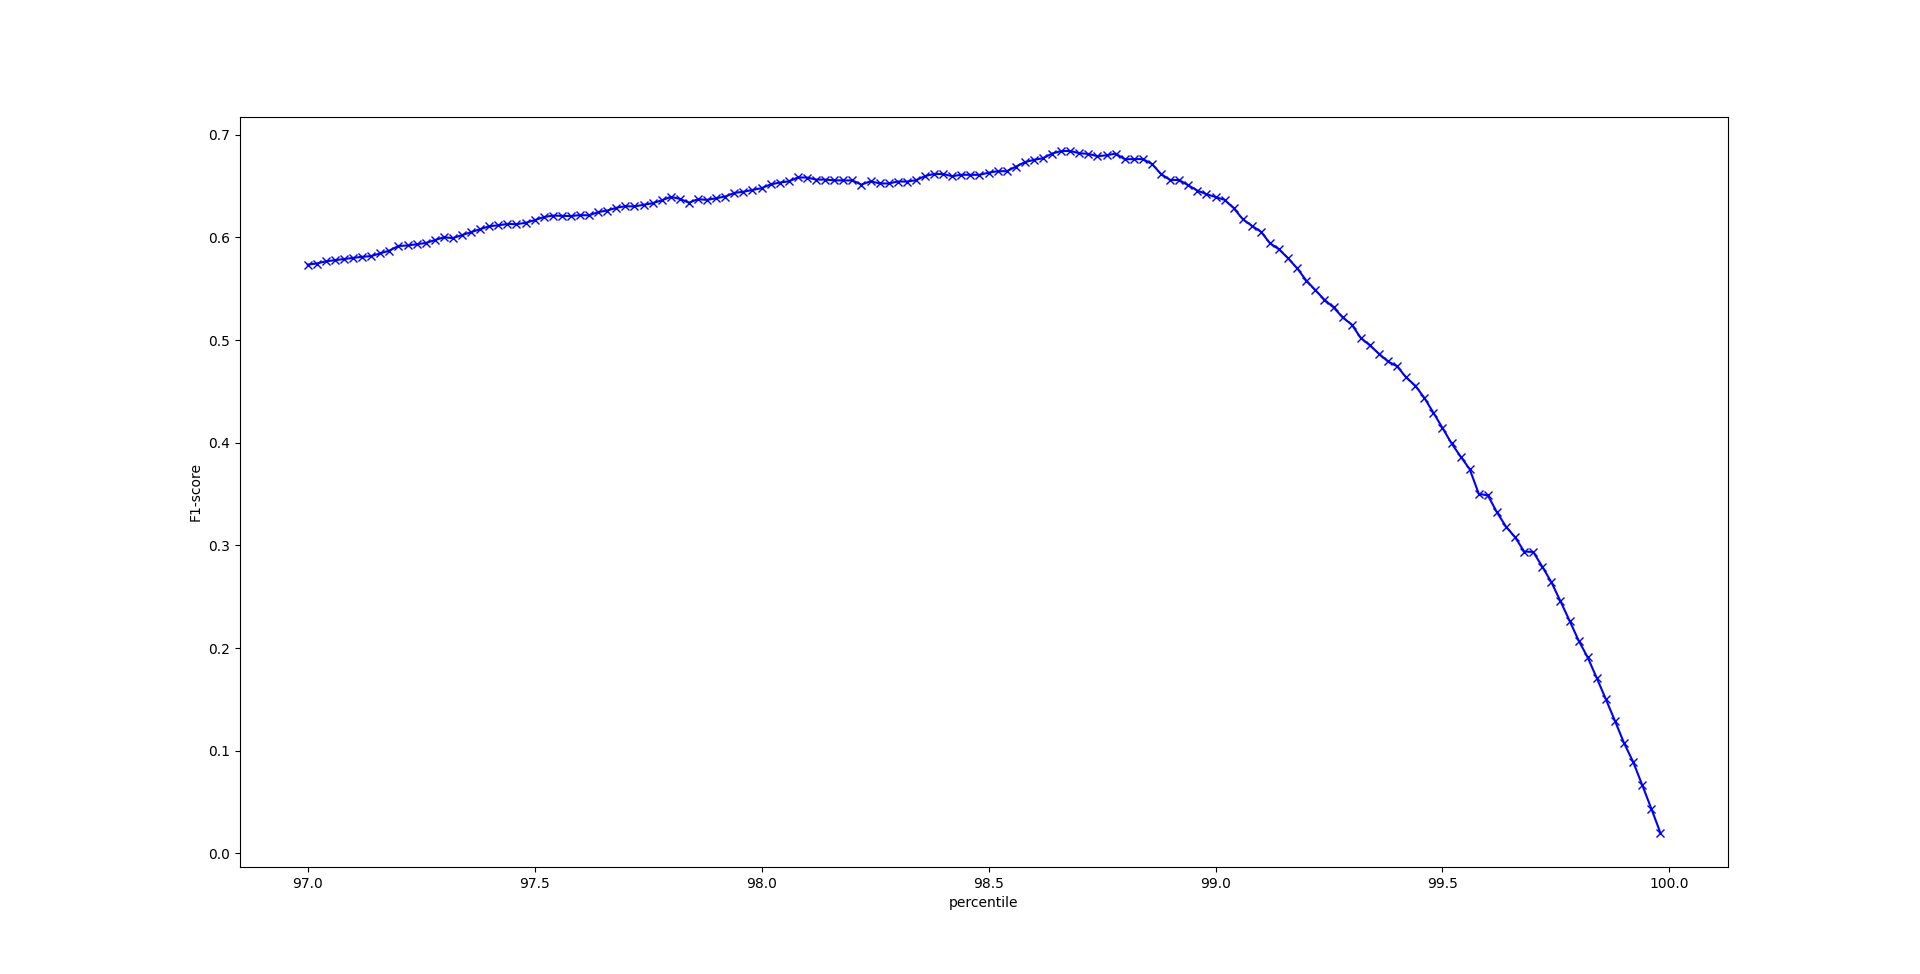
\includegraphics[width=1\textwidth]{images/credit-kmeans-f1.png}
\centering
\caption{Graf ovisnosti F1-mjere o percentilu udaljenosti za skup podataka o kreditnim karticama.}
\label{fig:credit-kmeans}
\end{figure}

Kako bi se definirali hiperparametri algoritma DBSCAN provedeno je pretraživanje po rešetci te su najveće vrijednosti F1-mjere dobivene za $\epsilon = 0.25$ i $minPts = 55$. Slika \ref{fig:credit-dbscan} prikazuje promjenu F1-mjere za različit minimalni broj točaka $minPts$ uz fiksnu udaljenost $\epsilon = 0.25$.

\begin{figure}[htb]
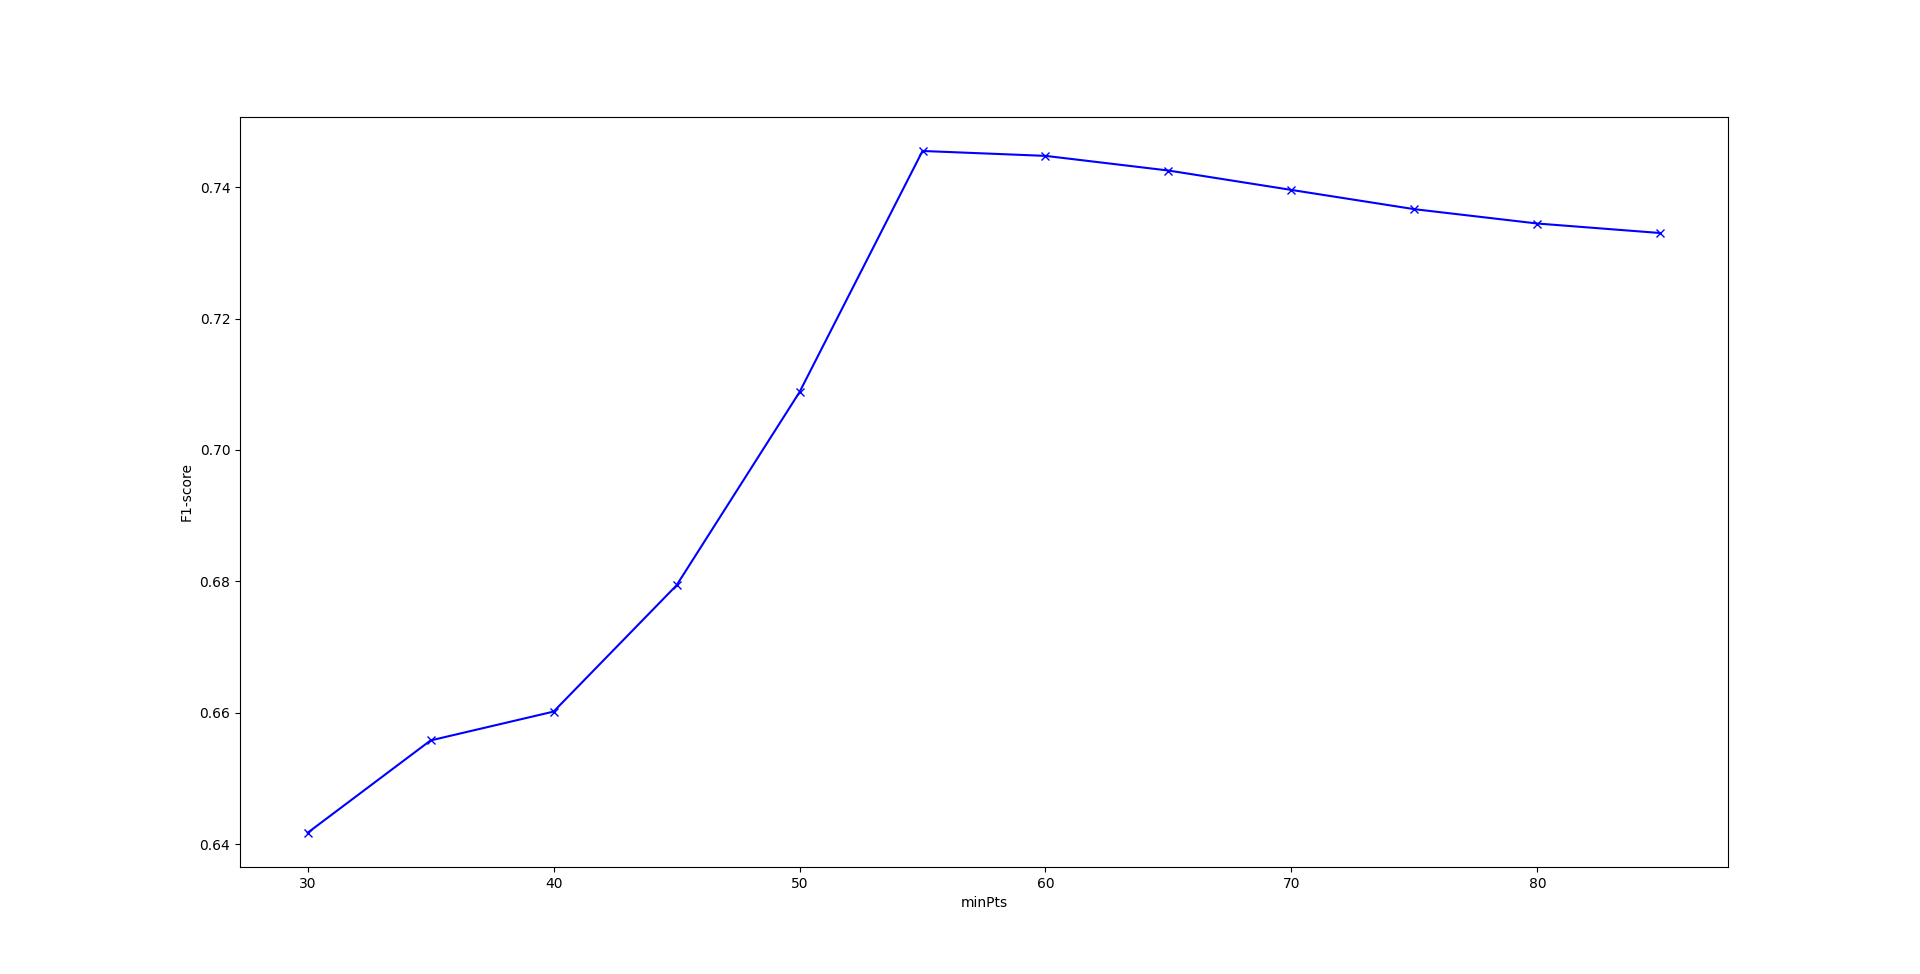
\includegraphics[width=1\textwidth]{images/credit-dbscan-f1.png}
\centering
\caption{Graf ovisnosti F1-mjere o minimalnom broju točaka $minPts$ uz $\epsilon = 0.25$ za skup podataka o kreditnim karticama.}
\label{fig:credit-dbscan}
\end{figure}

U slučaju modela Gaussove mješavine potrebno je odrediti percentil logaritamske izglednosti ispod kojeg se točke proglašavaju anomalijiama. Ovisnost F1-mjere o tom percentilu prikazana je na slici \ref{fig:credit-gauss} te je percentil 1.35 uzet kao granični percentil. Slučajno je i u algoritmu K-sredina i u modelu Gaussove mješavine odabran granični percentil koji proglašava jednak postotak primjera anomalijama odnosno 1.35\%.

\begin{figure}[htb]
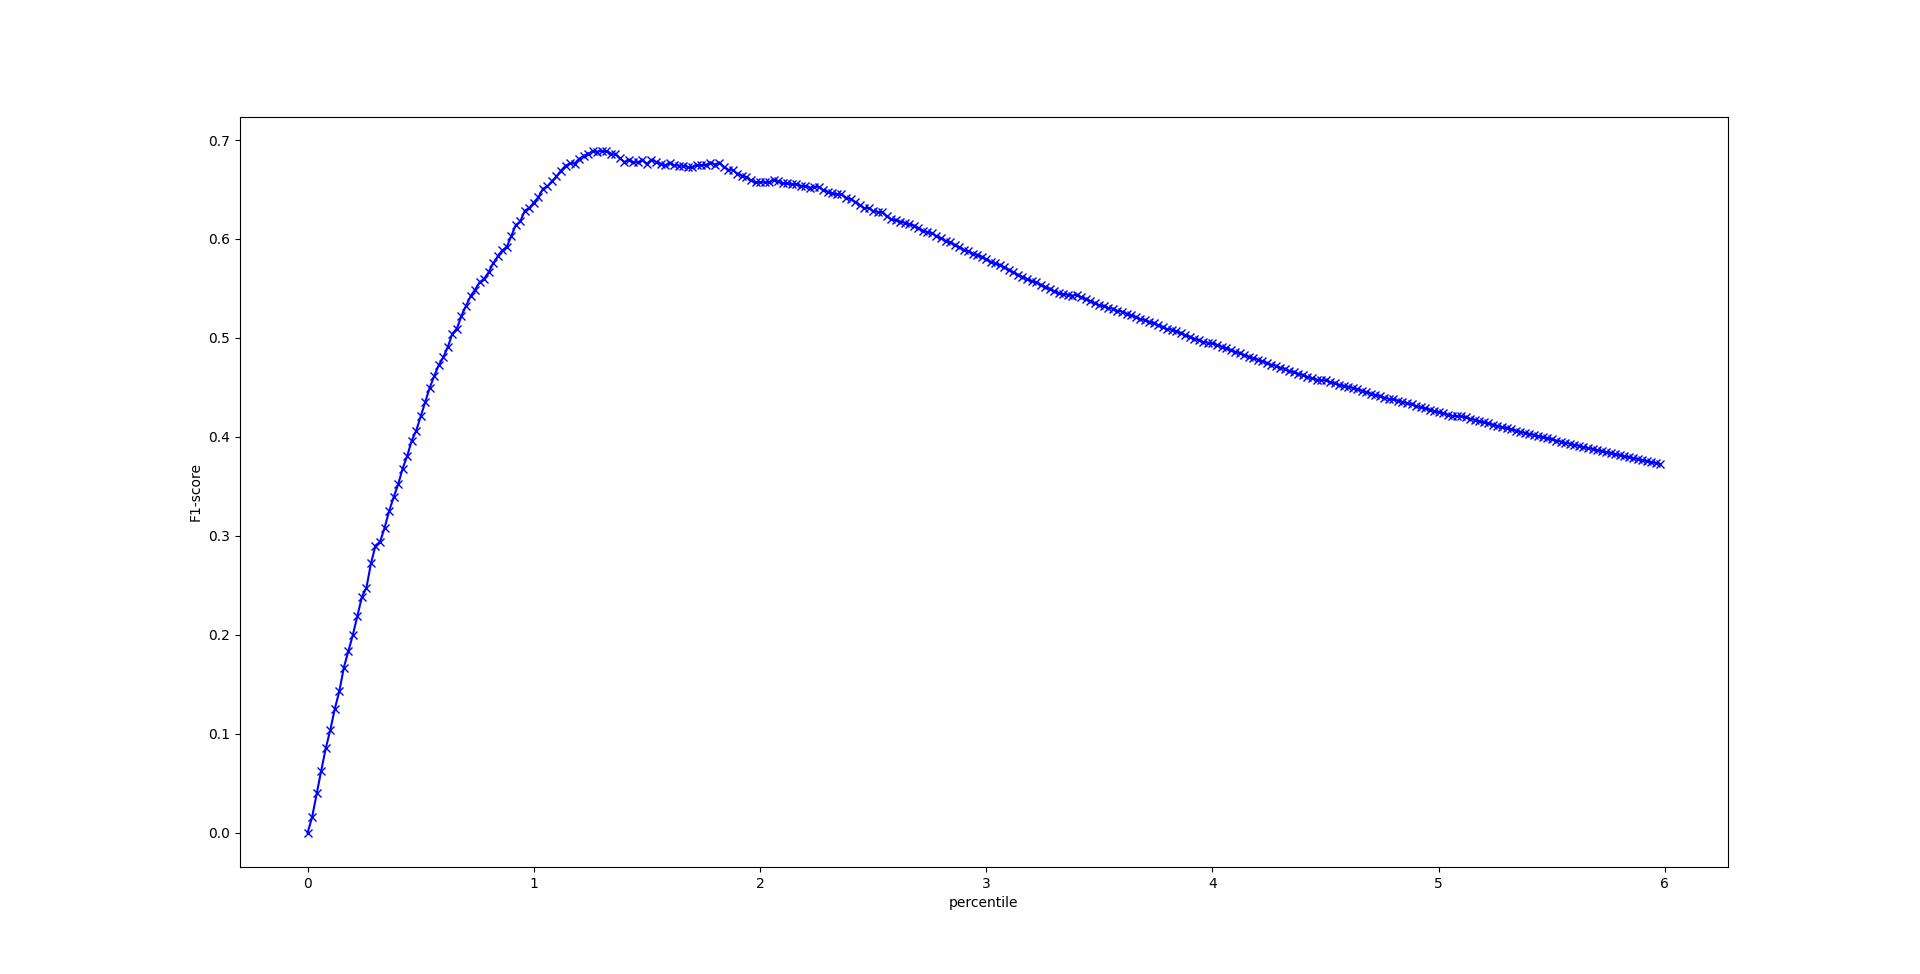
\includegraphics[width=1\textwidth]{images/credit-gauss-f1.png}
\centering
\caption{Graf ovisnosti F1-mjere o percentilu logaritamske izglednosti za skup podataka o kreditnim karticama.}
\label{fig:credit-gauss}
\end{figure}

\begin{table}[h!]
  \begin{center}
    \caption{Usporedba algoritama na skupu podataka o kreditnim karticama.}
    \label{tab:creditcard}
    \begin{tabular}{c|c|c|c} 
      & \textbf{K-sredine} & \textbf{DBSCAN}  & \textbf{Gaussova mješavina}\\
      \hline
      \textbf{Preciznost} & 0.774 & 0.721 & 0.771 \\
      \textbf{Odziv} & 0.615 & 0.753 & 0.613 \\
      \textbf{F1-mjera} & 0.685 & 0.737 & 0.683 \\
      \textbf{AUC mjera} & 0.806 & 0.874 & 0.805 \\
      \textbf{Randov indeks} & 0.981 & 0.982 & 0.981 \\
       \textbf{Koeficijent siluete} & 0.653 & 0.611 & 0.653 \\
       \textbf{Davies-Bouldin indeks} & 1.212 & 1.414 & 1.215 \\
     \end{tabular}
  \end{center}
\end{table}

\section{Detekcija upada u mrežu}

\subsection{Skup podataka \textit{U2R}}

\begin{figure}[htb]
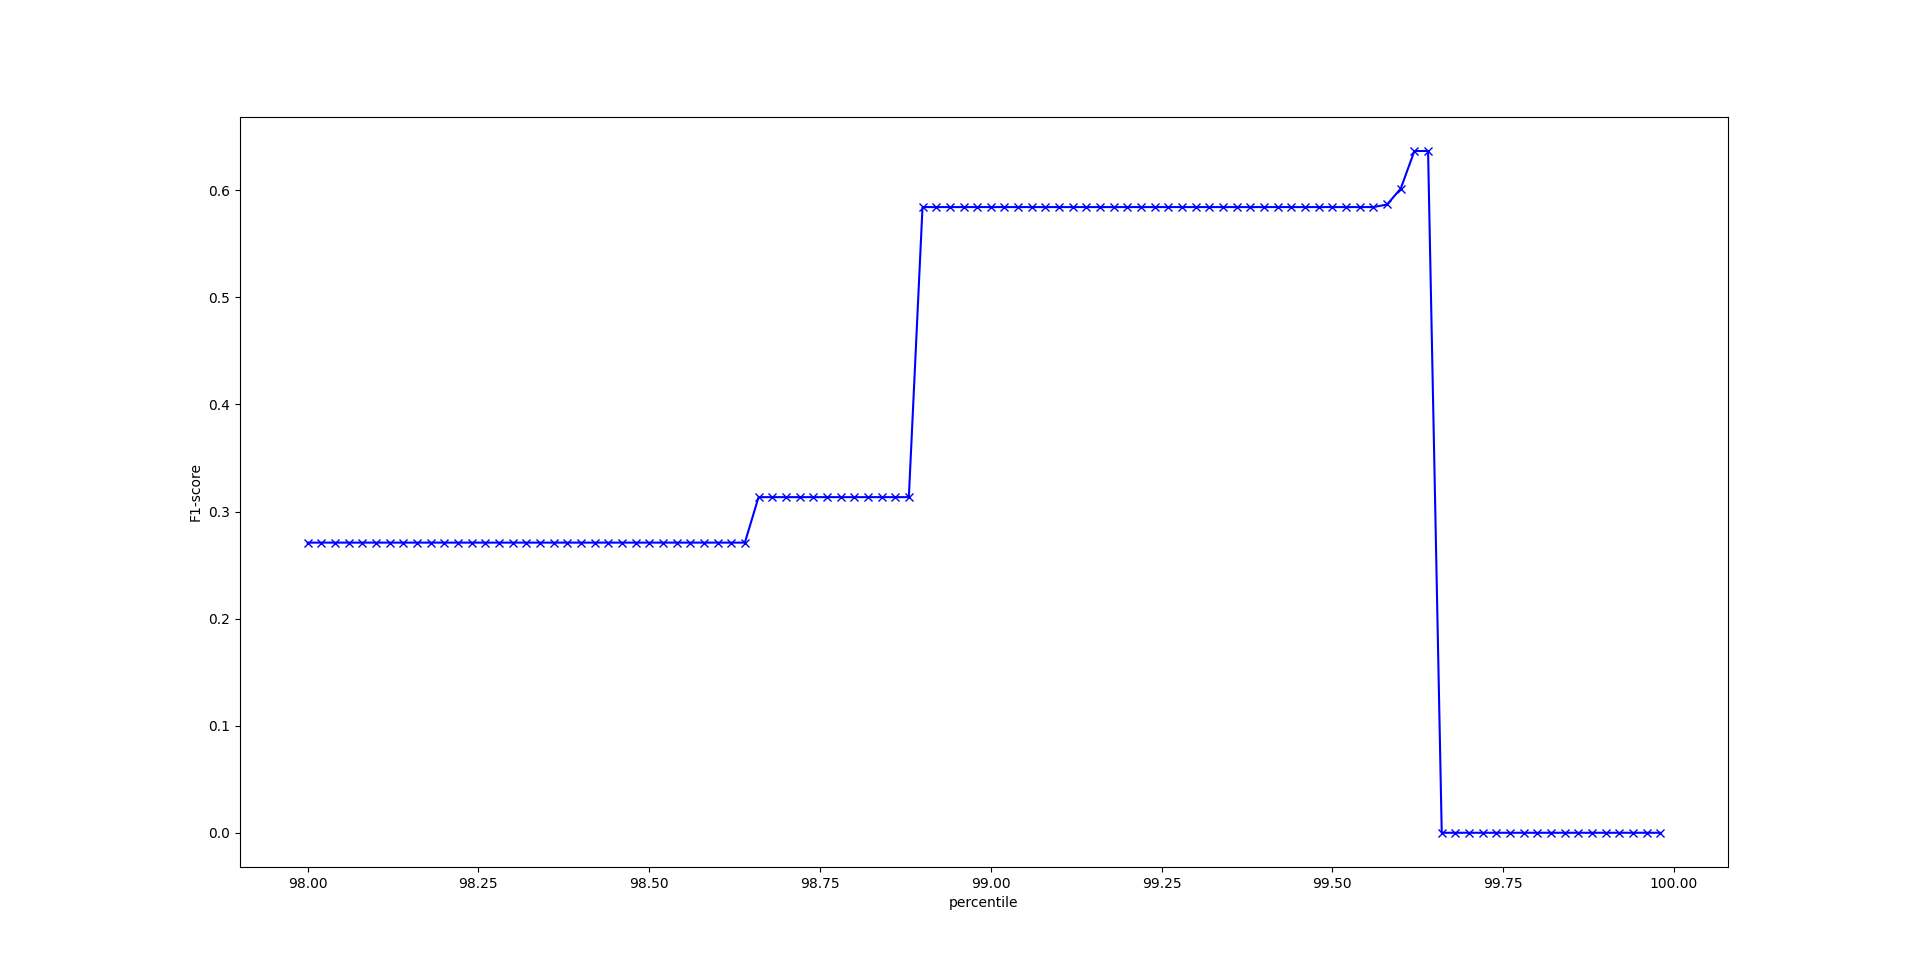
\includegraphics[width=1\textwidth]{images/u2r-kmeans-f1.png}
\centering
\caption{Primjer Gaussove mješavine za $K = 3$. Preuzeto s  \cite{GaussianMixtureExplained}}
\label{fig:u2r-kmeans}
\end{figure}

\begin{figure}[htb]
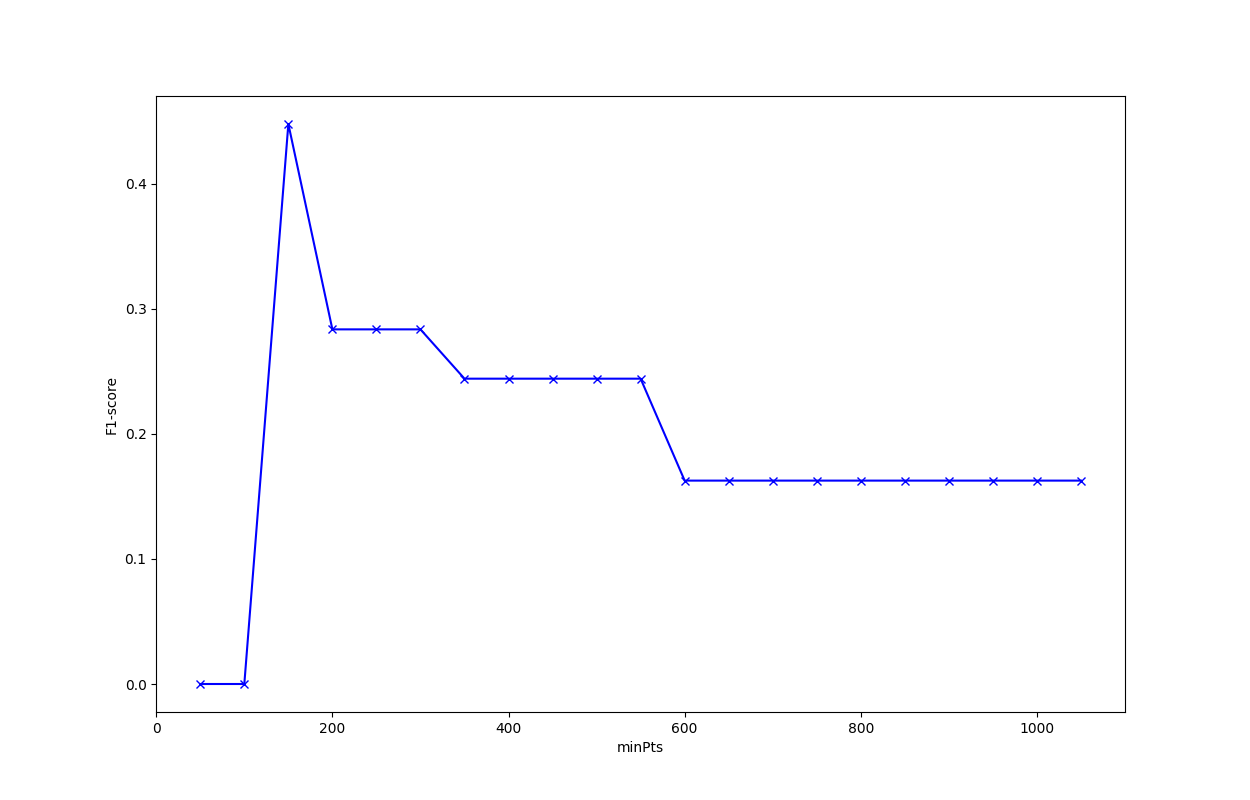
\includegraphics[width=1\textwidth]{images/u2r-dbscan-f1.png}
\centering
\caption{Primjer Gaussove mješavine za $K = 3$. Preuzeto s  \cite{GaussianMixtureExplained}}
\label{fig:u2r-dbscan}
\end{figure}

\begin{figure}[htb]
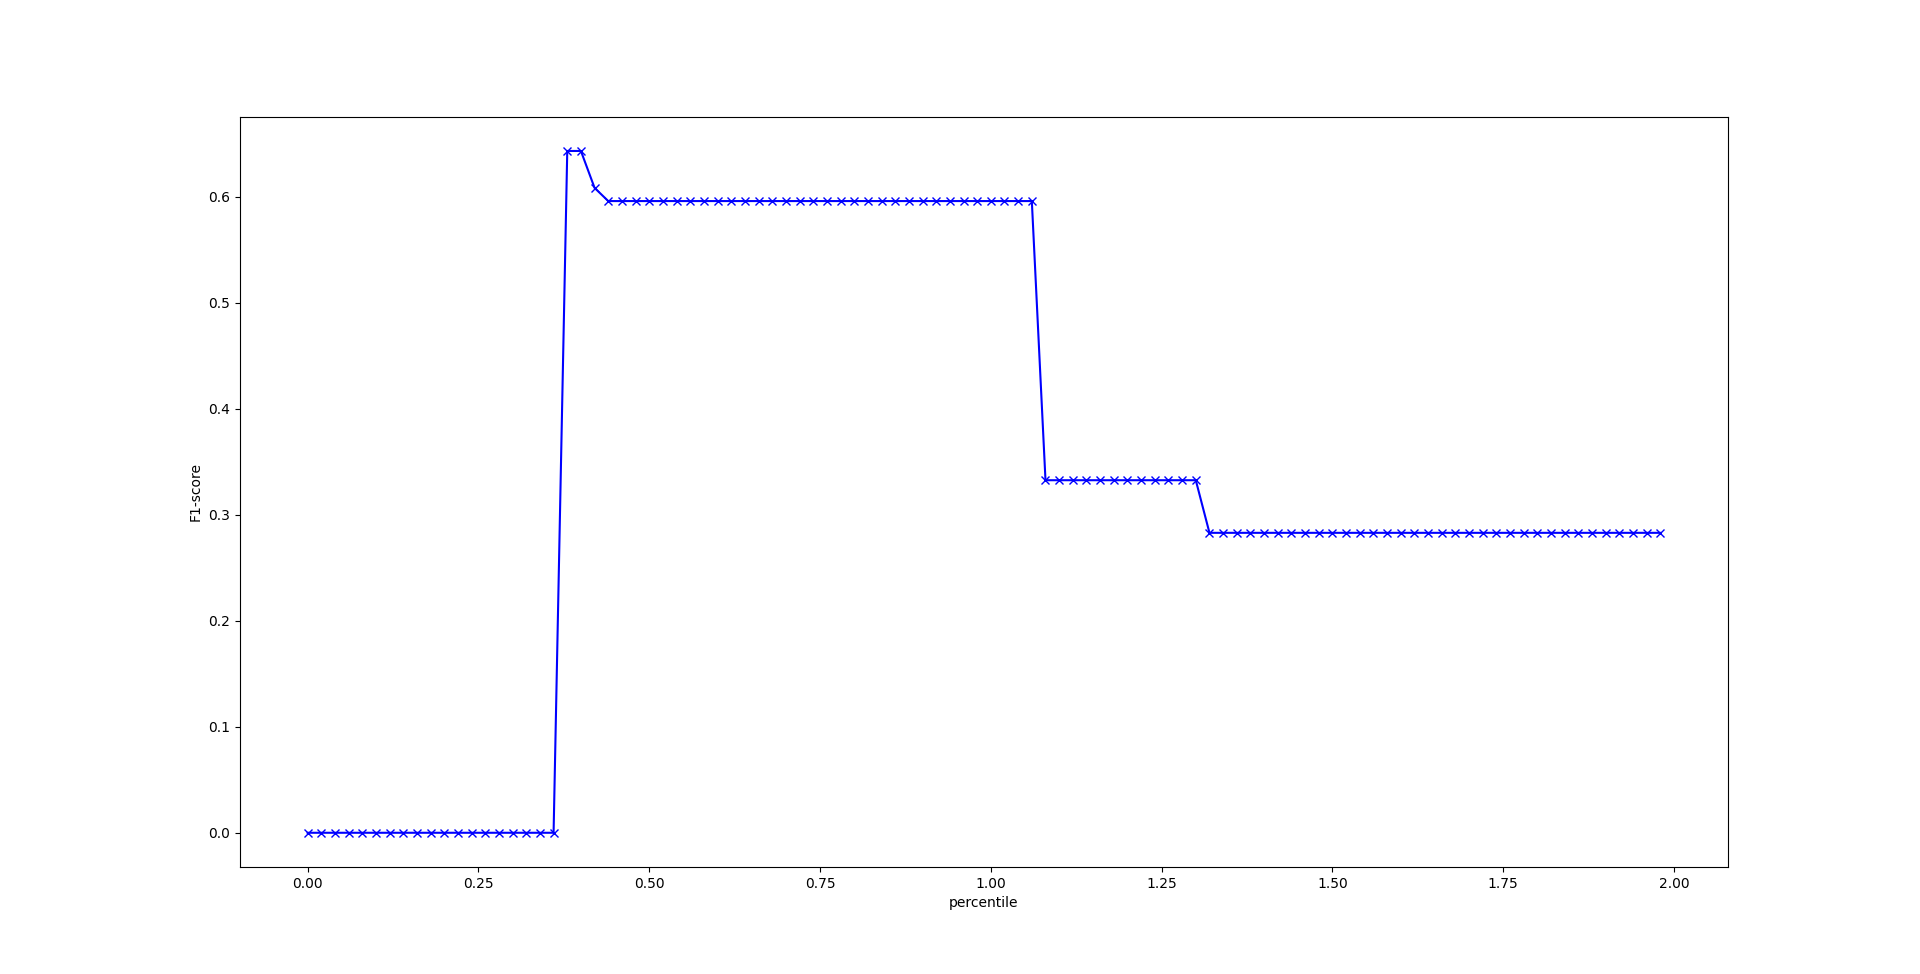
\includegraphics[width=1\textwidth]{images/u2r-gauss-f1.png}
\centering
\caption{Primjer Gaussove mješavine za $K = 3$. Preuzeto s  \cite{GaussianMixtureExplained}}
\label{fig:u2r-gauss}
\end{figure}

\subsection{Skup podataka \textit{Probe}}

\begin{figure}[htb]
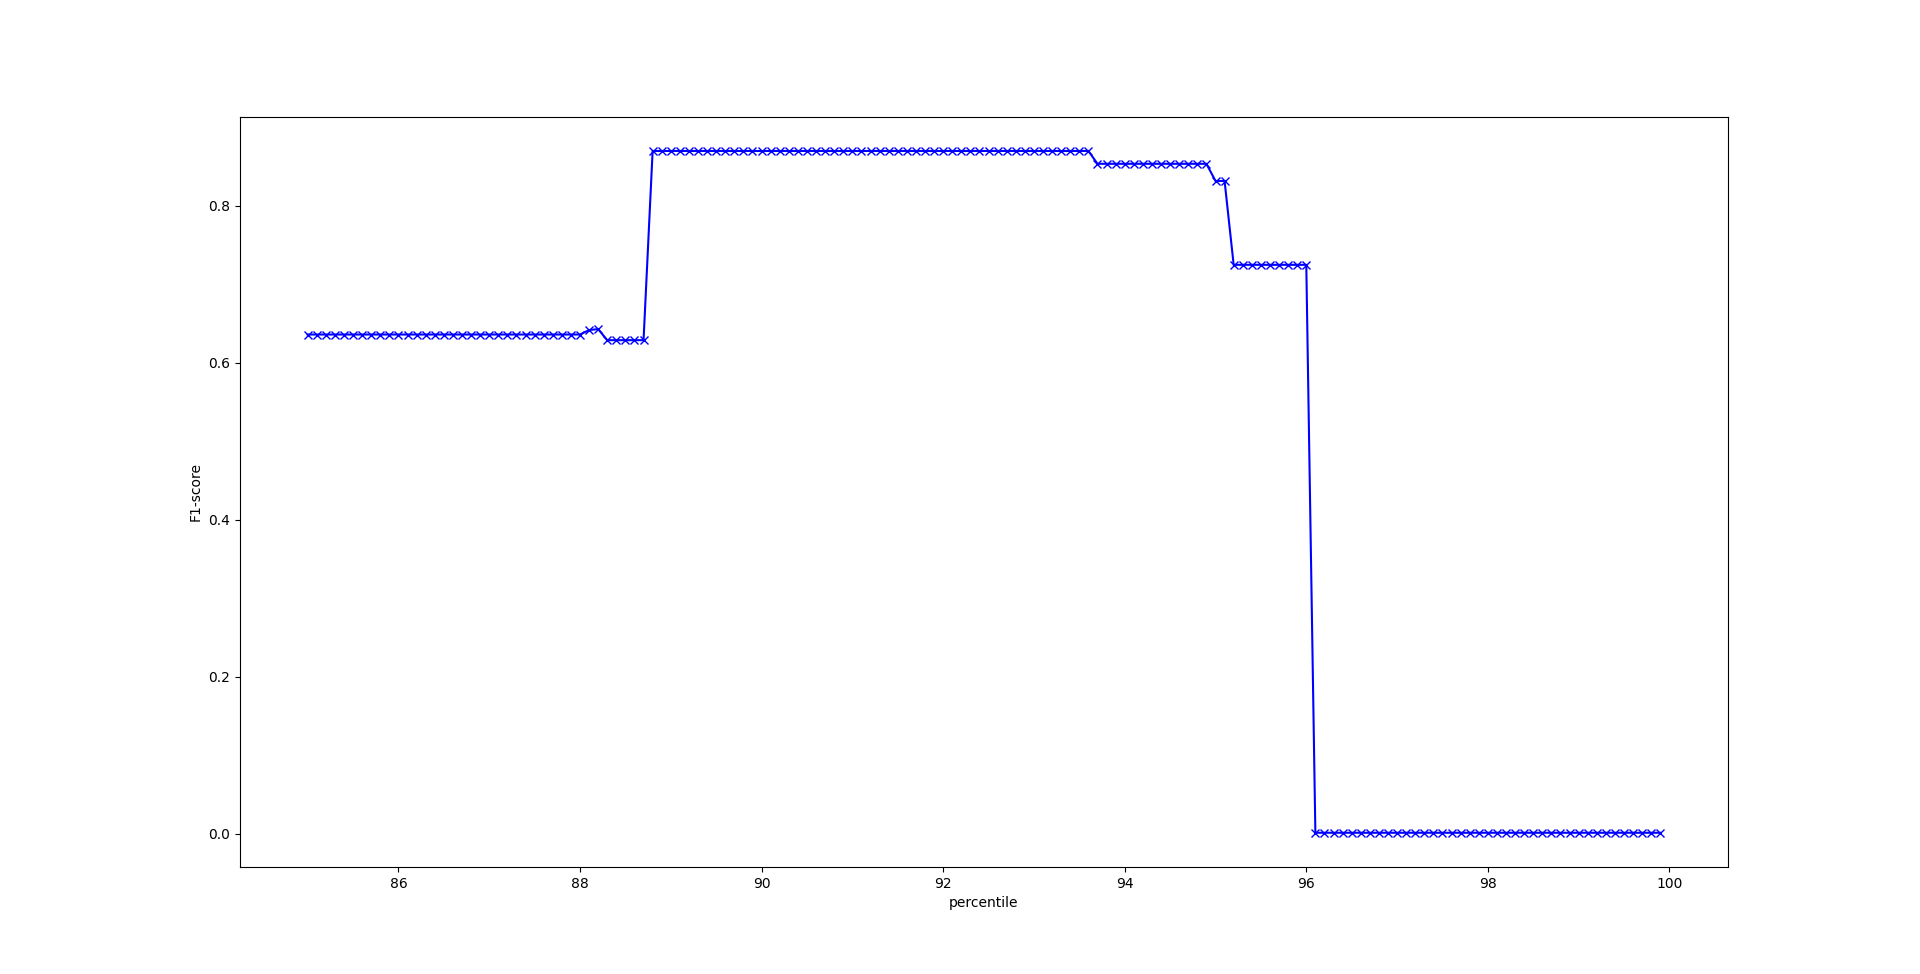
\includegraphics[width=1\textwidth]{images/probe-kmeans-f1.png}
\centering
\caption{Primjer Gaussove mješavine za $K = 3$. Preuzeto s  \cite{GaussianMixtureExplained}}
\label{fig:probe-kmeans}
\end{figure}

\begin{figure}[htb]
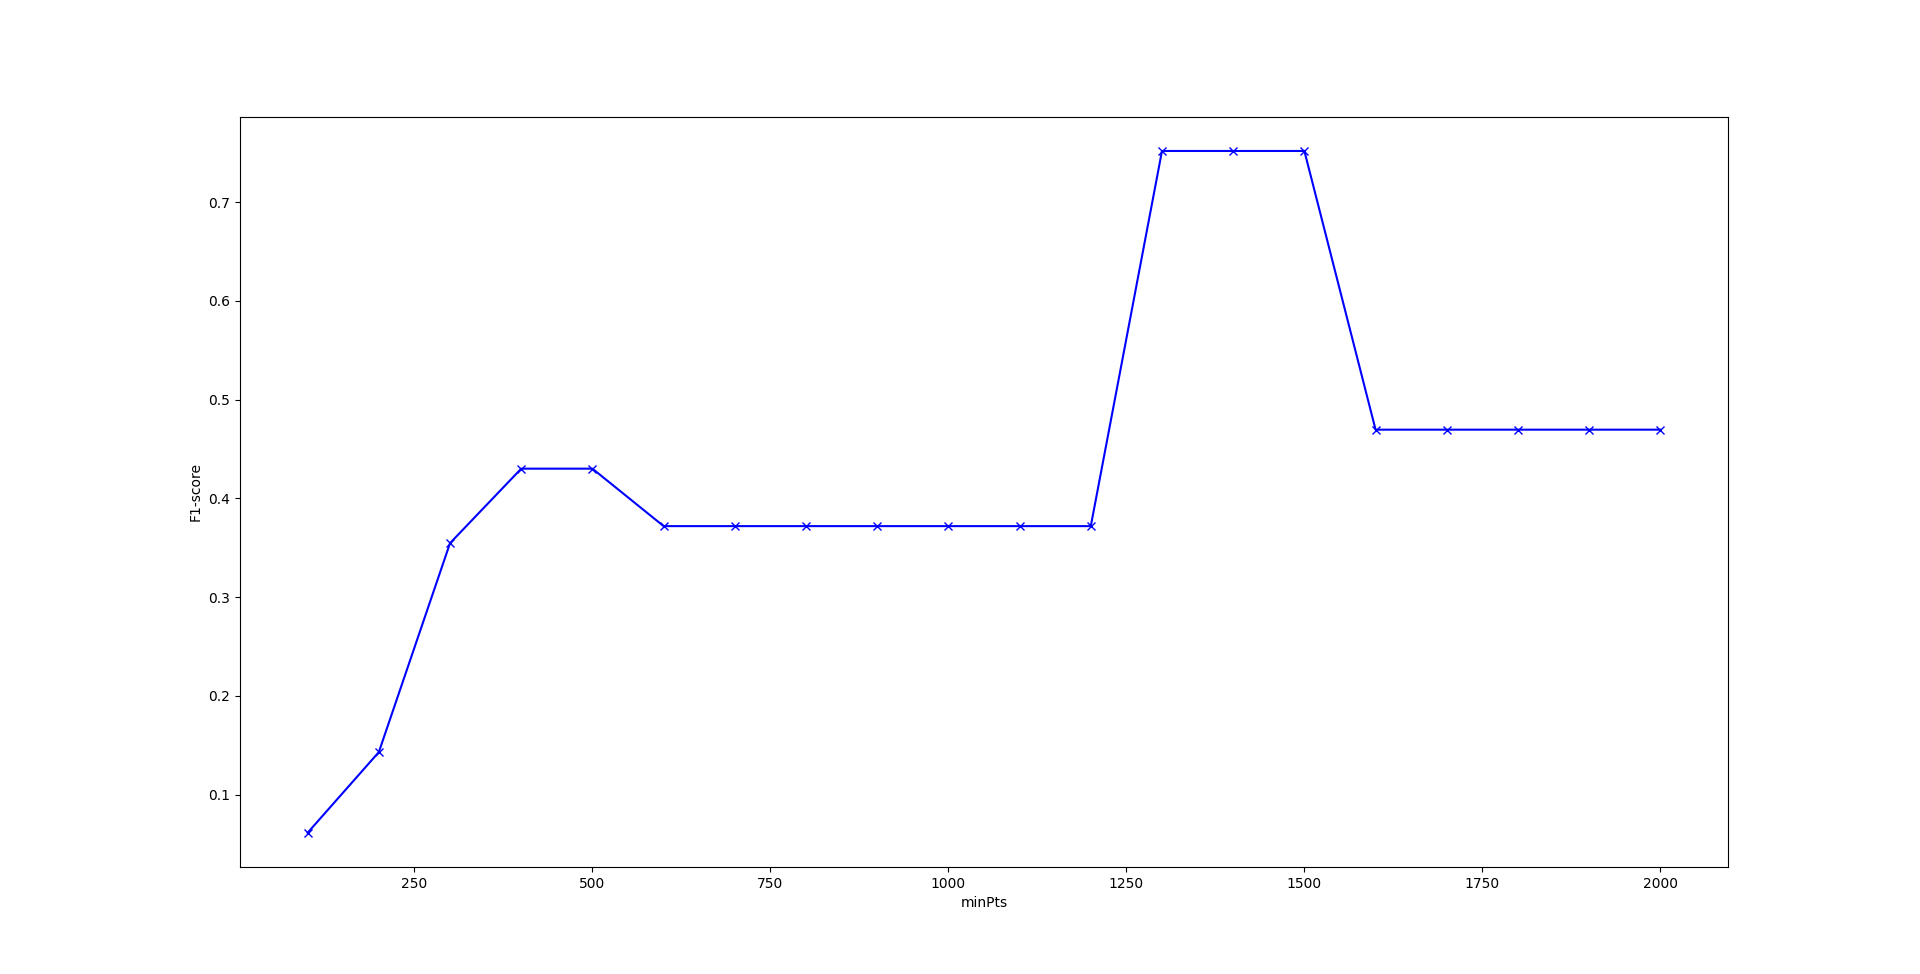
\includegraphics[width=1\textwidth]{images/probe-dbscan-f1.png}
\centering
\caption{Primjer Gaussove mješavine za $K = 3$. Preuzeto s  \cite{GaussianMixtureExplained}}
\label{fig:probe-dbscan}
\end{figure}

\begin{figure}[htb]
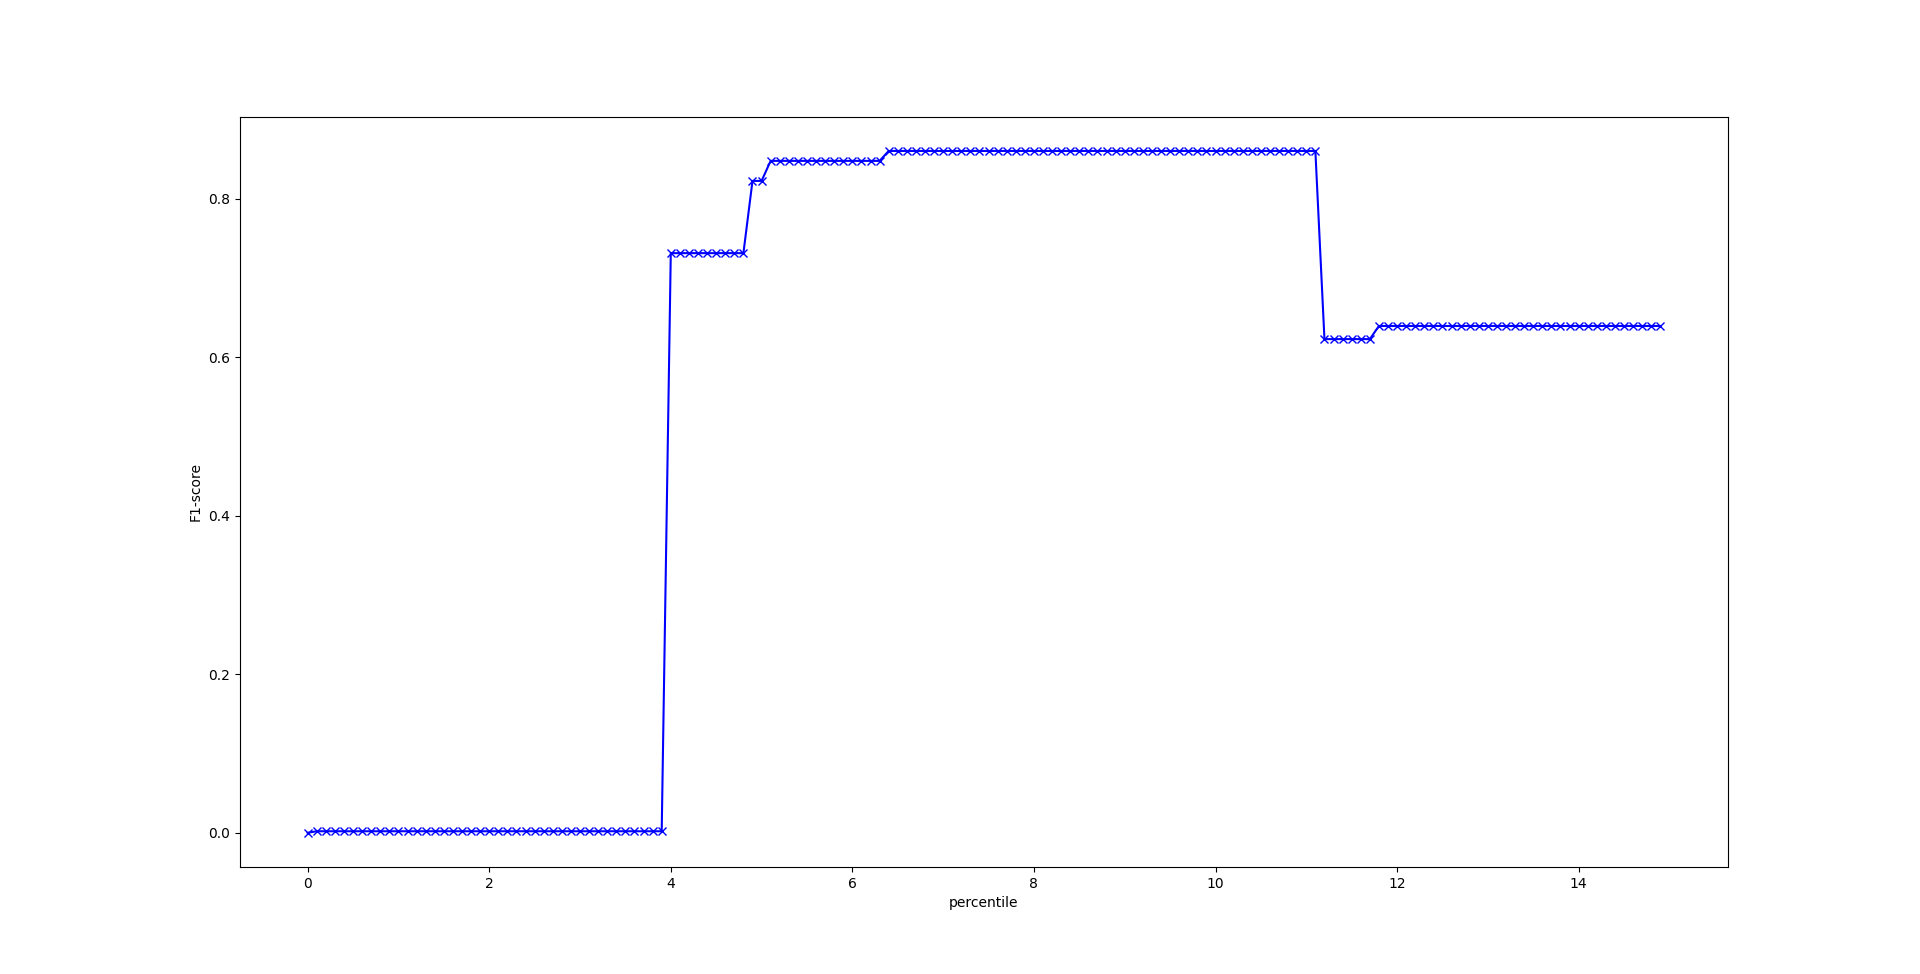
\includegraphics[width=1\textwidth]{images/probe-gauss-f1.png}
\centering
\caption{Primjer Gaussove mješavine za $K = 3$. Preuzeto s  \cite{GaussianMixtureExplained}}
\label{fig:probe-gauss}
\end{figure}

\section{Detekcija raka}

\begin{figure}[htb]
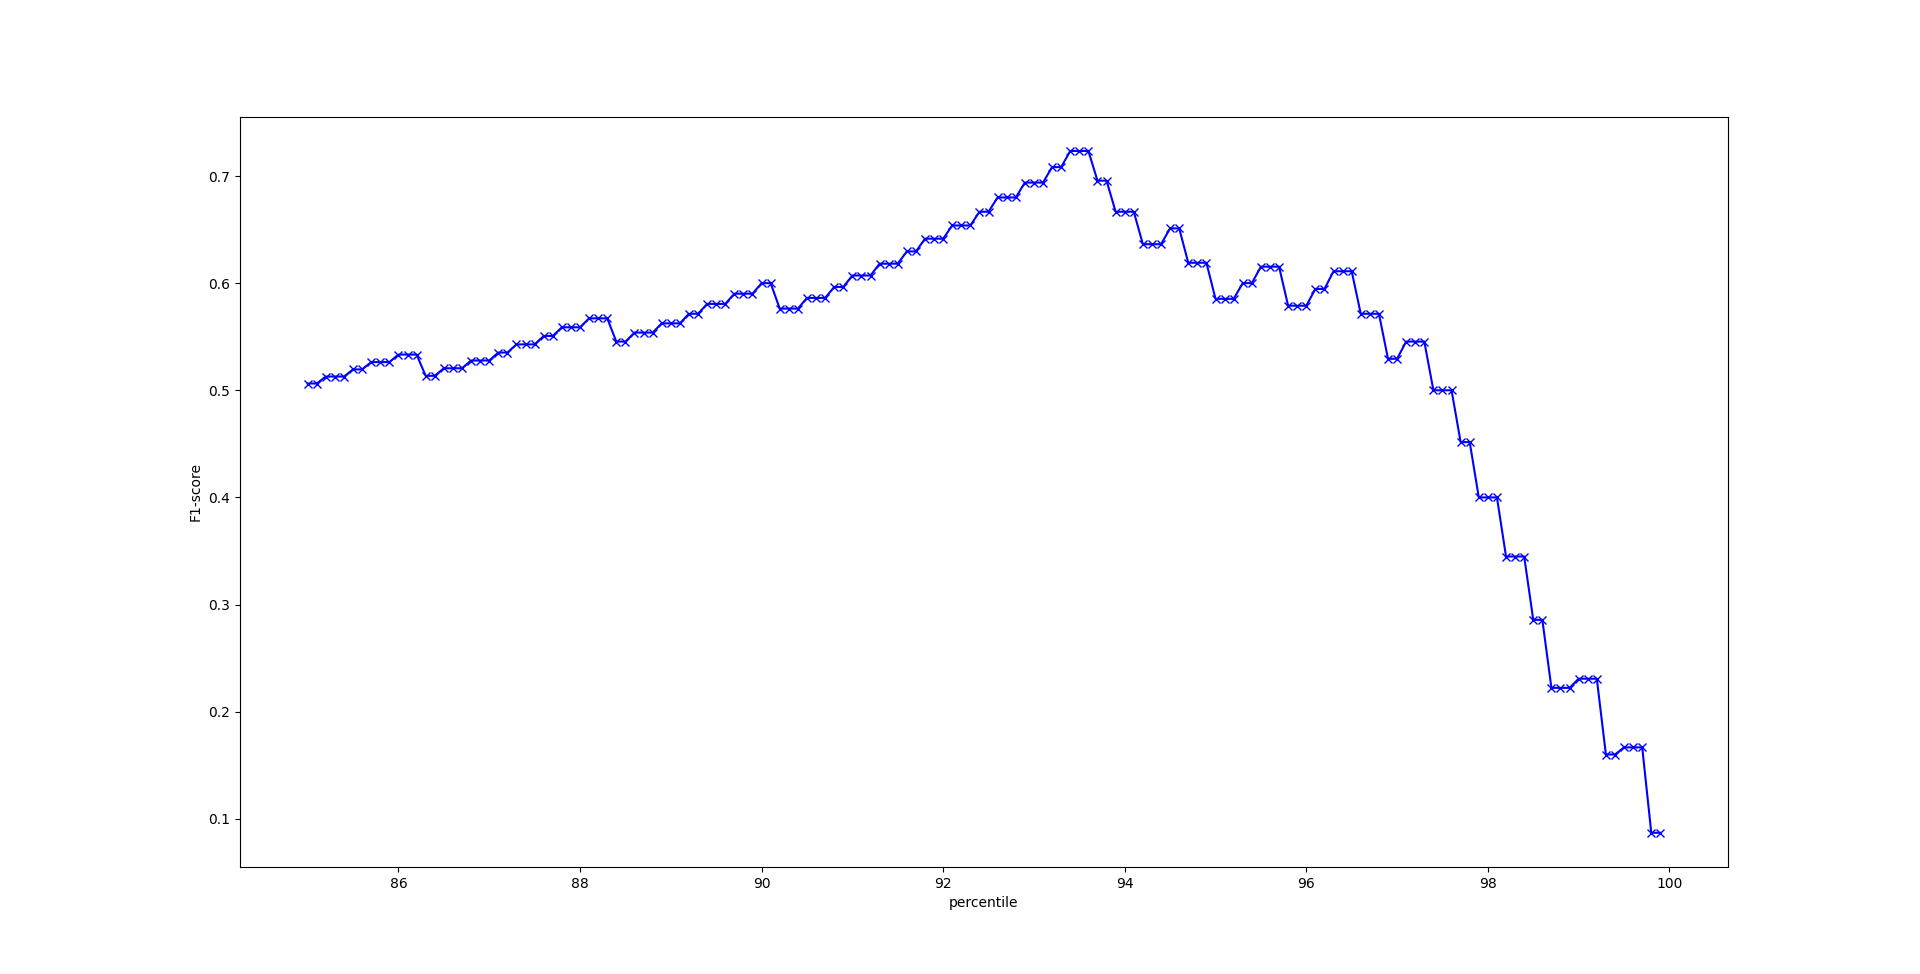
\includegraphics[width=1\textwidth]{images/cancer-kmeans-f1.png}
\centering
\caption{Primjer Gaussove mješavine za $K = 3$. Preuzeto s  \cite{GaussianMixtureExplained}}
\label{fig:cancer-kmeans}
\end{figure}

\begin{figure}[htb]
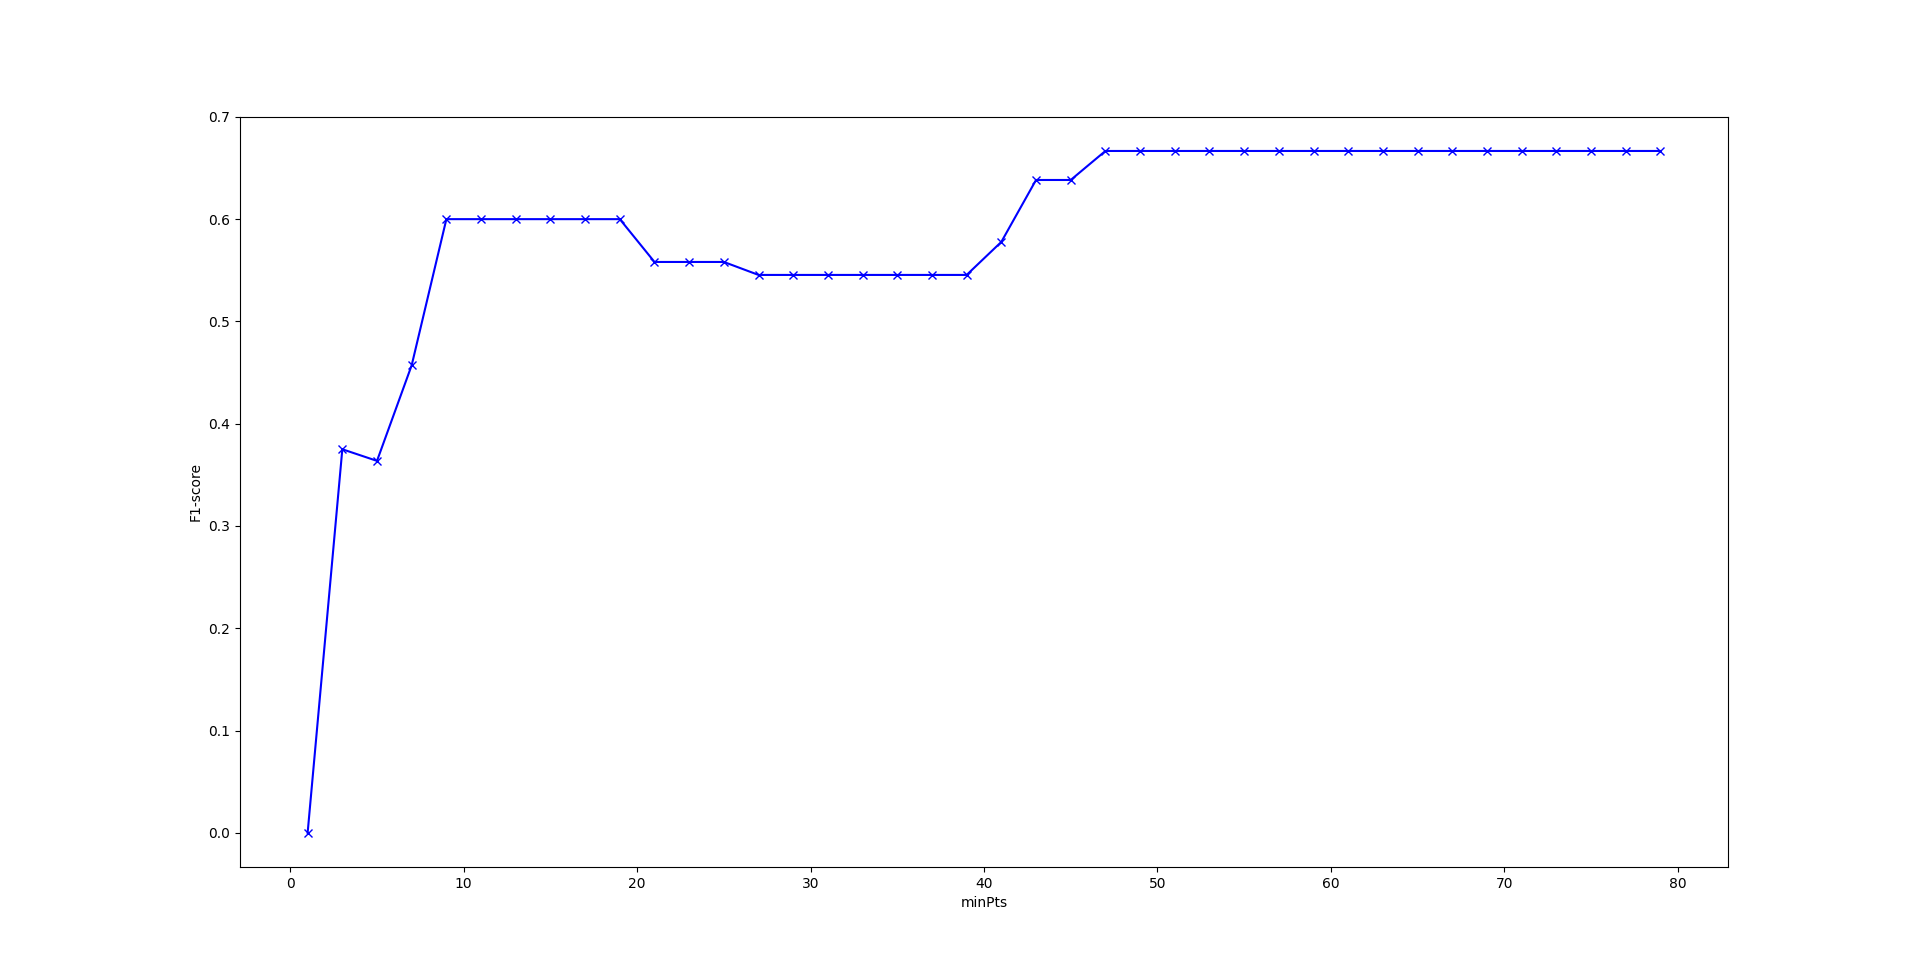
\includegraphics[width=1\textwidth]{images/cancer-dbscan-f1.png}
\centering
\caption{Primjer Gaussove mješavine za $K = 3$. Preuzeto s  \cite{GaussianMixtureExplained}}
\label{fig:cancer-dbscan}
\end{figure}

\begin{figure}[htb]
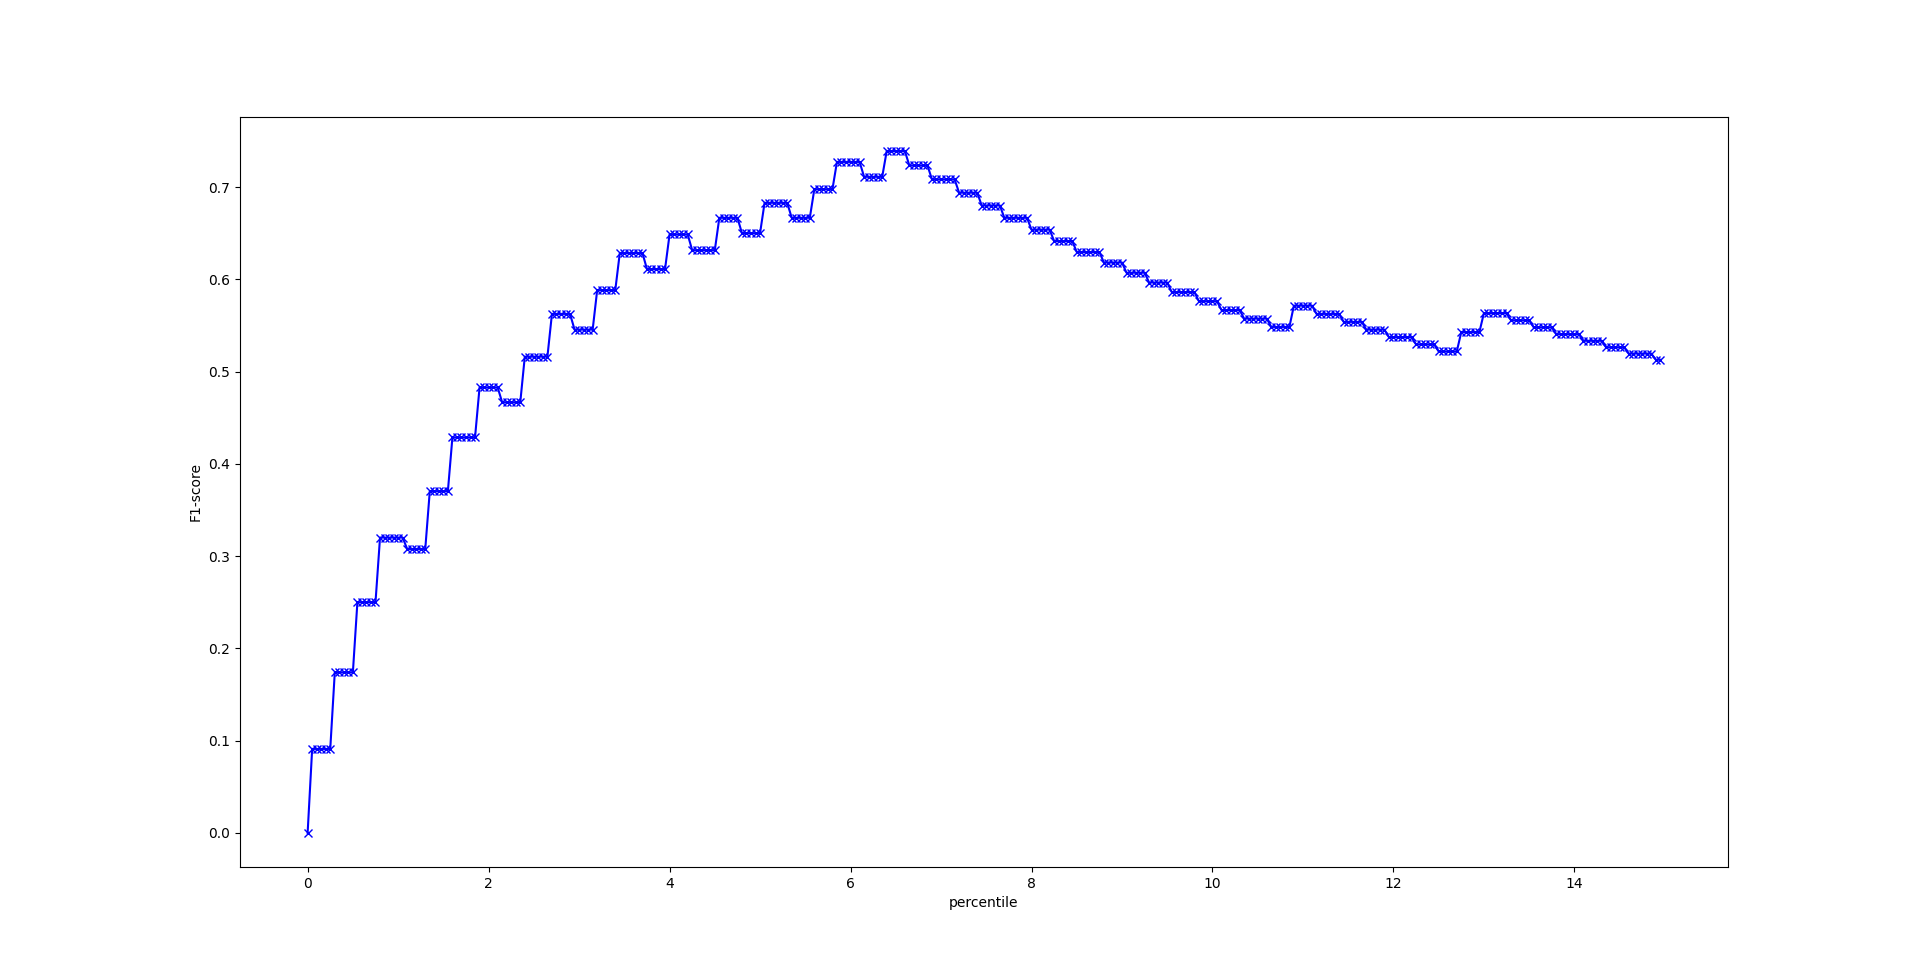
\includegraphics[width=1\textwidth]{images/cancer-gauss-f1.png}
\centering
\caption{Primjer Gaussove mješavine za $K = 3$. Preuzeto s  \cite{GaussianMixtureExplained}}
\label{fig:cancer-gauss}
\end{figure}

\chapter{Zaključak}
Zaključak.

\nocite{*}
\bibliography{literatura}
\bibliographystyle{fer}

\begin{sazetak}
Sažetak na hrvatskom jeziku.

\kljucnerijeci{Ključne riječi, odvojene zarezima.}
\end{sazetak}

% TODO: Navedite naslov na engleskom jeziku.
\engtitle{Title}
\begin{abstract}
Abstract.

\keywords{Keywords.}
\end{abstract}

\end{document}
